\RequirePackage{xr-hyper}
\documentclass[pdflatex,sn-mathphys-num]{sn-jnl}
\usepackage[utf8]{inputenc}
\usepackage{amsmath,amssymb,amsthm,mathtools,bm}
\usepackage{graphicx,booktabs,array,tabularx,float,longtable}
\usepackage{microtype,enumitem,needspace,placeins}
\usepackage{xurl}
\setlist{itemsep=2pt,topsep=4pt}
\setlength{\emergencystretch}{2em}
\renewcommand{\topfraction}{0.9}
\renewcommand{\bottomfraction}{0.8}
\renewcommand{\textfraction}{0.1}
\renewcommand{\floatpagefraction}{0.8}
\setlength{\parindent}{1.2em}
\theoremstyle{thmstyleone}
\newtheorem{theorem}{Theorem}[section]
\newtheorem{proposition}[theorem]{Proposition}
\newtheorem{lemma}[theorem]{Lemma}
\newtheorem{corollary}[theorem]{Corollary}
\theoremstyle{thmstylethree}
\newtheorem{definition}[theorem]{Definition}
\newtheorem{assumption}[theorem]{Assumption}
\newtheorem{remark}[theorem]{Remark}
\newcounter{algorithm}
\newenvironment{method}[1]{\refstepcounter{algorithm}\par\medskip
  \noindent\textbf{Algorithm \thealgorithm. #1}\par\smallskip\hrule\smallskip}
  {\smallskip\hrule\medskip}
\newcommand{\R}{\mathbb R}
\newcommand{\norm}[1]{\left\lVert#1\right\rVert}
\newcommand{\rank}{\operatorname{rank}}
\newcommand{\diag}{\operatorname{diag}}
\newcommand{\dist}{\operatorname{dist}}
\newcommand{\Argmin}{\operatorname*{arg\,min}}
\newcommand{\cA}{\mathcal A}
\newcommand{\cB}{\mathcal B}
\newcommand{\eps}{\varepsilon}
\hypersetup{pdftitle={Tangent Excess and Persistent Difference-of-Convex Regularization for Nonconvex QCQPs},pdfauthor={Francois Akoa}}

\externaldocument[][nocite]{Akoa_LazyQCQP_20261111_R24_Supplement}[Akoa_LazyQCQP_20261111_R24_Supplement.pdf]

\usepackage{xcolor}
\newenvironment{scaledtable}[1][tbp]{\begin{tableorg}[#1]\centering}{\end{tableorg}}
% Plain page numbers, without the diagnostic literal in the distributed style.
\makeatletter
\def\ps@plain{\let\@mkboth\@gobbletwo\let\@oddhead\@empty\let\@evenhead\@empty
  \def\@oddfoot{\hfil\thepage\hfil}\let\@evenfoot\@oddfoot}
\makeatother
\hypersetup{hidelinks,hypertexnames=false,bookmarksdepth=3}
\begin{document}
\title{Tangent Excess and Persistent Difference-of-Convex Regularization for Nonconvex QCQPs}
\author*[1]{\fnm{Fran\c{c}ois} \sur{Akoa}}\email{francois.akoa@maatai-lab.com}
\affil[1]{\orgname{MAATAI-LAB}, \orgaddress{\country{France}}}
\abstract{Componentwise convexification can impose a local convergence cost
on nonconvex quadratically constrained quadratic programs (QCQPs).
We derive a lower bound on the relative tangent excess forced by
negatively curved components with positive Lagrangian weights.
QCQP examples attain this bound. We characterize corrections confined
to normal directions. Established
sensitivity formulas convert this excess $\kappa$ into the factor
$\kappa/(1+\kappa)$, reproduced by controlled trajectories. LazyQCQP reuses
difference-of-convex corrections, refines components and preserves signed
quadratic-equality curvature. A specified filter algorithm has stationary
accumulation points under explicit assumptions. At a regular
Karush--Kuhn--Tucker (KKT) limit, a sufficiently small curvature threshold
makes additional diagonal regularization unnecessary. On 4,078 QCQPs,
six configurations are compared with Ipopt using an independent
original-KKT certificate. With MUMPS for both solvers, the baseline
LazyQCQP configuration (R3) certifies 98.9\% of 1,037 cases with quadratic
inequalities and no quadratic equality, versus 97.1\% for monotone Ipopt
with certificate-matched stopping targets. On 797 mixed cases with both
quadratic constraint types, the rates are 82.8\% versus 53.1\%.
MA27 reverses the first ordering (96.0\% versus 97.2\%) but preserves
the second (83.2\% versus 55.0\%). For instances certified by both solvers,
with both process times above one second, the median ratio of R3 process
time to Ipopt process time with MUMPS is 0.34 in the first class and
0.48 in the mixed class. A controlled radio-beamforming ablation shows
that removing quadratically implied bounds lowers attained objectives
but can reduce certificate counts. On 12 instances, reuse
preserves trajectories and reduces median paired process times
by approximately 15\% with either linear solver.}
\keywords{nonconvex QCQP, difference of convex programming,
structured regularization, persistent curvature, quadratic equalities,
local convergence rate}
\pacs[MSC Classification]{90C26, 90C30, 90C51, 65K05}
\maketitle
\pagestyle{plain}
\raggedbottom
\section{Introduction}\label{sec:introduction}
Componentwise convexification can change the local geometry even when
the original constrained second-order curvature is favourable. Feasible
motion depends on the multiplier-weighted excess on the active tangent
space. We derive a lower bound on the excess forced by componentwise
convexity, attain it within the class of quadratically constrained
quadratic programs (QCQPs), and characterize corrections confined to
normal directions.

Fixed component Hessians make QCQPs a natural setting for controlling
this distortion. If $q$ has Hessian $Q$, a correction $M\succeq0$ with
$Q+M\succeq0$ defines the convex upper model
$m_q(y;x)=q(y)+\tfrac12(y-x)^TM(y-x)$.
Its value and gradient match $q$ at $x$, and the same correction remains
valid at subsequent iterates. LazyQCQP retains these corrections,
refines selected components, and embeds them in a sparse primal--dual
Newton system. Quadratic equalities retain their original equations
and signed Lagrangian curvature. The algorithm proceeds as follows:

\begin{method}{LazyQCQP at a glance}\label{alg:lazy}
\begin{enumerate}[leftmargin=1.7em]
\item At the current iterate, assess component corrections and select
      those to construct or refine.
\item Reuse valid corrections and update the selected components,
      preserving the required upper-model conditions.
\item Form the primal--dual Newton equations for these models with signed
      equality curvature. Compute a direction using the specified
      inertia and accuracy safeguards.
\item Restrict trial steps to keep slacks and inequality multipliers
      positive. Test acceptance with the original objective and constraints.
\item After acceptance, update the iterate, the models and the barrier and
      safeguard parameters. Otherwise keep the iterate and apply the
      recovery rule. Stop at the original KKT tolerance or the work
      limits, and independently check the final point.
\end{enumerate}
\end{method}

The lower bound quantifies the tangent excess forced by admissible
convexifications. At a stationary point with independent active gradients, strict
complementarity and positive definite reduced Lagrangian Hessian,
let $H_*$ be the original Lagrangian Hessian. For each nonzero
active tangent direction $v$, convexified components $q_i$ with
nonnegative Lagrangian weights $w_i$ force
\[
 \kappa\geq
 \frac{\sum_i w_i[-v^T\nabla^2q_i(x_*)v]_+}{v^TH_*v}.
\]
Here $\kappa$ is the largest tangent ratio of weighted correction to
original curvature; the objective has weight one. Established
sensitivity formulas for the model solution map convert this excess into the spectral
factor $\kappa/(1+\kappa)$. A QCQP example attains the bound. A
complementary necessary and sufficient criterion determines whether
convexification can leave tangent motion unchanged. It includes a
range condition when the tangent restriction is singular. Correction
rank alone therefore gives little information about local distortion.

The filter algorithm LazyQCQP-F has a global stationarity guarantee under
explicit boundedness, regularity, restoration and barrier-continuation
assumptions. If its iterates converge to a KKT point satisfying the stated
regularity conditions, a small enough curvature threshold eventually removes
the additional diagonal regularization. The local rate also requires a
limiting model, full steps and vanishing forcing errors. Persistent diagonal
regularization adds a quantified penalty. Exact minimization of convex
models gives feasibility, descent and residual guarantees under stronger
assumptions. The benchmark evaluates complete algorithms with their own
globalization and recovery rules.

Global QCQP methods combine feasible incumbents with lower bounds from
reformulation--linearization \citep{SheraliTuncbilek1992}, moment relaxations
\citep{Lasserre2001} and spatial branch-and-bound
\citep{TawarmalaniSahinidis2005}. LazyQCQP supplies complementary stationary candidates. Certified original
feasibility makes such a point a valid incumbent and its objective value
an upper bound.

LazyQCQP denotes the persistent-correction framework: R3 is the
benchmark reference with reusable support-based corrections, HH, HS, SH and SS are complete
alternative policies, and $SS_0$ is a scalar control. Within each regime, we compare their certificate counts, attained
objectives and computational cost.

The experiments test the geometric predictions on controlled
QCQPs, then compare six configurations with MA27 and MUMPS against
Ipopt using the same linear solvers on 4,078 problems from 28
collections. Common coefficients, raw initial points, budgets and an
independent original-KKT test allow comparisons of coverage,
objectives and paired times. Results are organized by quadratic
constraint structure. Collection-level and equal-weight summaries
examine corpus composition. The configuration comparisons combine several algorithmic choices.
Separate experiments vary refinement, bound removal or correction reuse
while keeping the other relevant choices fixed.

Tangent upper models originate in inner approximation
\citep{MarksWright1978} and appear in DC algorithms and the
convex--concave procedure \citep{LeThiPhamDinh2018,LippBoyd2016}.
For quadratic problems, DC methods have been studied on balls and spheres
\citep{PhamDinhLeThi1996,PhamDinhLeThi1998}, over intersections of
ellipsoids \citep{LeThi2000Ellipsoids}, and with linear constraints
\citep{LeThiPhamDinhYen2011}. IPDCA already combines DC regularization
of indefinite QP Hessians with primal--dual interior-point equations
\citep{Akoa2005Thesis,PhamDinhLeThiAkoa2008}. Here the extension to QCQPs
uses persistent component corrections, preserves signed equality curvature,
and analyzes their multiplier-weighted tangent excess within a specified
filter algorithm.
Exact penalties and convex inner approximations provide frameworks for
general DC constraints
\citep{LeThiPhamDinhHuynh2012,LeThiHuynhPhamDinh2014,LuSunZhou2022}.
For general QCQPs, Park and Boyd's working paper
\emph{General Heuristics for Nonconvex Quadratically Constrained Quadratic
Programming} (2017, \href{https://arxiv.org/abs/1703.07870}{arXiv:1703.07870})
develops a local Suggest-and-Improve framework that includes a penalty
convex--concave procedure.
Global approaches also exploit the choice of DC decomposition
\citep{VanVoorhisAlKhayyal2003,ZhengSunLi2011}.
Sequential quadratic constraint and moving-balls methods supply related
curved models \citep{FukushimaLuoTseng2003,Solodov2004,AuslenderShefiTeboulle2010}.
Here fixed component Hessians make corrections reusable, and their
multiplier-weighted tangent excess quantifies a local cost of valid
componentwise convexification.

The local sensitivity relation is established for majorization--minimization
\citep[Section~6.1]{HunterLange2004} and constrained sequential convex
programming \citep[Theorem~4.5]{MessererBaumgaertnerDiehl2021}.
The contribution is a lower bound on the excess forced by convexity,
QCQP examples attaining this bound, and the normal-space criterion. The global analysis uses the filter
framework of \citet{WachterBiegler2005Global}, connecting bounded
persistent corrections to a lower bound on tangent curvature and determining
when additional diagonal regularization becomes unnecessary. These results connect model
geometry to the Newton iteration under the assumptions stated for
each convergence result.
\section{Componentwise convexification and tangent excess}\label{sec:model}
Consider
\begin{equation}\label{eq:problem}
 \min_{x\in\R^n} f(x)\quad\text{subject to}\quad
 g_i(x)\leq0\ (i=1,\ldots,m),\qquad
 h_j(x)=0\ (j=1,\ldots,p).
\end{equation}
Every function is a quadratic polynomial; affine functions are included
as quadratics with zero Hessian. Bounds may be included among the affine
inequalities. We write
\[
 f(x)=\tfrac12 x^TQ_0x+c_0^Tx+d_0,\qquad
 g_i(x)=\tfrac12 x^TQ_ix+c_i^Tx+d_i,
\]
and denote $\nabla^2h_j$ by $H_j$. All Hessians are symmetric. No
positive semidefiniteness is assumed for the original functions.
Unsubscripted vector norms are Euclidean, and matrix norms are their
induced spectral norms unless stated otherwise.
The Jacobians $J_g$ and $J_h$ have constraint gradients as rows.

With inequality multipliers $\lambda\geq0$ and unrestricted equality
multipliers $\nu$, the Lagrangian and its Hessian are
\begin{align}
 L(x,\lambda,\nu)&=f(x)+\lambda^Tg(x)+\nu^Th(x),\label{eq:lagrangian}\\
 H_L(\lambda,\nu)&=Q_0+\sum_i\lambda_iQ_i+\sum_j\nu_jH_j.
 \label{eq:lagrangian-hessian}
\end{align}
The KKT conditions are primal feasibility, $\lambda\geq0$,
$\nabla_xL=0$, and $\lambda_i g_i=0$. Throughout, a reported KKT point means a first order stationary point;
second order sufficient conditions establish local minimality.

We assess all final points using the same original, unscaled residual
\begin{equation}\label{eq:kkt-residual}
 \mathcal R(x,\lambda,\nu)=\max\left\{
 \norm{[g(x)]_+}_\infty,\norm{h(x)}_\infty,
 \norm{\nabla_xL}_\infty,
 \max_i|\lambda_i g_i(x)|,\norm{[-\lambda]_+}_\infty\right\}.
\end{equation}
The maximum over an empty constraint set is zero. When bounds are kept
explicitly, their multipliers and complementarity terms are included in
this definition. Multipliers for absent bounds are zero. The numerical dual residual
combines the stationarity norm and multiplier sign violations. Function
scaling can be useful during a solve, with original units restored for
the common final-point test.

\subsection{Tangent and normal curvature}
Let $x_*$ be a KKT point and let $\cA_*=\{i:g_i(x_*)=0\}$ denote
the active inequality indices. Let $A_*$ contain the gradients of these
inequalities and of all equality constraints as rows. Under
linear independence of these gradients (LICQ), take an orthonormal basis
$Z$ of $\ker A_*$. Under strict complementarity, the second order
sufficient condition is
\begin{equation}\label{eq:sosc}
 H_T:=Z^TH_L(\lambda_*,\nu_*)Z\succ0.
\end{equation}
Tangent directions leave the active constraint values unchanged to first order.
An ambient-space correction may be large while its restriction to this
space is zero. Conversely, even a small-rank correction may strongly
affect the only tangent direction. This distinction will determine the
local rate.


% Main Section 2, after the QCQP and Lagrangian definitions, before models
% and detailed algorithms. This replaces (rather than duplicates) the old
% lower-bound corollary. Keep its historic label for existing links, but
% change textual references from 'Corollary' to 'Theorem'.
\subsection{Unavoidable tangent excess}
\label{sec:tangent-excess-bound}
Let $(x_*,\lambda_*,\nu_*)$ be a KKT point and let $A_*$ contain the
gradients of its active inequalities and equalities, including active
bounds. Take an orthonormal basis $Z$ of $\ker A_*$, assumed here to
have positive dimension, and set
\[
 H_*=\nabla^2_{xx}L(x_*,\lambda_*,\nu_*),\qquad
 H_T=Z^TH_*Z\succ0.
\]
The bound below concerns curvature at this point; it does not require an
iteration or a model-solution map. Write $q_0=f$, $q_i=g_i$,
$w_0=1$ and $w_i=\lambda_{i,*}\geq0$ for
$i\in\mathcal A_*$. For positive semidefinite component corrections
$M_i$, $i\in\{0\}\cup\mathcal A_*$, define their weighted excess by
\begin{equation}\label{eq:tangent-excess-definition}
 \begin{split}
 E_*&=M_0+\sum_{i\in\mathcal A_*}\lambda_{i,*}M_i,\\
 E_T&=Z^TE_*Z,\\
 \kappa&=\lambda_{\max}(H_T^{-1/2}E_TH_T^{-1/2})
       =\max_{\substack{v\in\ker A_*\\v\ne0}}
          \frac{v^TE_*v}{v^TH_*v}.
 \end{split}
\end{equation}
Thus, $\kappa$ is the largest ratio of added DC curvature to original
Lagrangian curvature over nonzero tangent directions.

\begin{theorem}[A lower bound on tangent excess]
\label{cor:smooth-convexification-obstruction}
With the preceding definitions, let
$\mathcal C\subseteq\{0\}\cup\mathcal A_*$ be any set of components
whose corrected Hessians are positive semidefinite:
\[
 \nabla^2q_i(x_*)+M_i\succeq0\qquad(i\in\mathcal C).
\]
For every nonzero $v\in\ker A_*$,
\begin{equation}\label{eq:smooth-convexification-obstruction}
 \kappa\geq
 \frac{\displaystyle\sum_{i\in\mathcal C}
          w_i[-v^T\nabla^2q_i(x_*)v]_+}{v^TH_*v}.
\end{equation}
In particular, negative component curvature along a tangent direction,
with a positive corresponding weight, forces $\kappa>0$ whenever
that component is convexified. The bound is attained within the QCQP
class for every prescribed positive value of $\kappa$.
\end{theorem}
\begin{proof}
For $i\in\mathcal C$, positive semidefiniteness of $M_i$ and
$\nabla^2q_i(x_*)+M_i$ gives
\[
 v^TM_iv\geq[-v^T\nabla^2q_i(x_*)v]_+.
\]
All other contributions to $v^TE_*v$ are nonnegative. Multiplying by
$w_i$, summing and using the Rayleigh quotient in
\eqref{eq:tangent-excess-definition} proves the bound.

To show that the bound is attained, choose $a,c>0$ and consider
\begin{equation}\label{eq:attainment-qcqp}
 \min_{s,t}\;s+\frac{a+c}{2}t^2
 \quad\text{subject to}\quad -s-\frac c2t^2\leq0.
\end{equation}
The objective is at least $at^2/2$ on the feasible set, so the unique
solution is $(0,0)$, with multiplier $\lambda_*=1$. Its tangent is
$\operatorname{span}\{(0,1)\}$ and $H_T=a$. Retain the exact
objective, $M_0=0$, and use $M_1=\operatorname{diag}(0,c)$ for the
inequality. The corrected inequality Hessian is zero, $E_T=c$ and
both sides of \eqref{eq:smooth-convexification-obstruction} equal
$c/a$. Choosing $c/a$ gives any prescribed positive $\kappa$.
\end{proof}

The construction attains the bound within the QCQP class by choosing
the instance and its correction. The pointwise argument also applies
to $C^2$ components, using their Hessians at $x_*$. The statement concerns curvature. Under the additional regularity and
first-order model consistency hypotheses of Theorem~\ref{thm:smooth-anchored-map}, the
established sensitivity formula converts $\kappa$ into the local
spectral factor $\kappa/(1+\kappa)$. A positive lower bound $\omega$
in \eqref{eq:smooth-convexification-obstruction} then forces that
factor to be at least $\omega/(1+\omega)$. This is a worst-direction
linearized bound; individual trajectories may be faster. Convexity of
the objective model is required only if the objective is included in
$\mathcal C$; an exact objective remains admissible otherwise.

\Needspace{10\baselineskip}
\subsection{Tangent preserving convexification}
\label{sec:normal-correction}
Rank describes the size of the matrix representation; restriction to
feasible tangent directions describes its effect on the local iteration.
The following criterion separates these questions. It is a specialization of the positive semidefinite
Schur complement criterion \citep{HornJohnson2013}, used here to interpret quadratic models.

\begin{proposition}[Convexification by a normal correction]
\label{prop:normal-correction}
Let $Q$ be symmetric, let $Z$ have orthonormal columns spanning a
specified tangent space, and let $N$ complete $Z$ to an orthogonal
basis. Write
\[
 C=Z^TQZ,\qquad B=Z^TQN,\qquad D=N^TQN.
\]
There exists $M\succeq0$ such that
$Q+M\succeq0$ and $Z^TMZ=0$ if and only if
\begin{equation}\label{eq:normal-correction-condition}
 C\succeq0,\qquad \operatorname{range}(B)
                         \subseteq\operatorname{range}(C).
\end{equation}
Whenever these conditions hold and $N$ has at least one column, one may take
\[
 M=\gamma NN^T,\qquad
 \gamma\geq\max\{0,\lambda_{\max}(B^TC^\dagger B-D)\},
\]
where $C^\dagger$ is the pseudoinverse. If $C\succ0$,
the range condition holds automatically and $C^\dagger=C^{-1}$.
If there are no normal directions, the condition reduces to
$Q\succeq0$ and $M=0$. If there are no tangent directions, it
reduces to a positive scalar shift $\gamma I$ of $Q$.
\end{proposition}
\begin{proof}
For a positive semidefinite matrix $M$, $Z^TMZ=0$ implies
$M^{1/2}Z=0$, hence $MZ=0$. Therefore every such correction has the
form $M=NAN^T$ with $A\succeq0$. In the orthogonal basis $[Z,N]$,
\[
 Q+M\ \longleftrightarrow
 \begin{bmatrix}C&B\\B^T&D+A\end{bmatrix}.
\]
Positive semidefiniteness forces $C\succeq0$. For
$z\in\ker C$, the vector $(z,0)$ has zero quadratic form and
must lie in the null space of the full positive semidefinite matrix;
thus $B^Tz=0$. This is exactly the range condition in
\eqref{eq:normal-correction-condition}.
Conversely that range condition and $C\succeq0$ give the
completion of squares identity
\[
 \begin{pmatrix}u\\v\end{pmatrix}^{\!T}
 \begin{bmatrix}C&B\\B^T&D+A\end{bmatrix}
 \begin{pmatrix}u\\v\end{pmatrix}
 =(u+C^\dagger Bv)^TC(u+C^\dagger Bv)
   +v^T(D+A-B^TC^\dagger B)v.
\]
Choosing $A=\gamma I$ as stated makes both terms nonnegative.
Empty spaces are handled by dropping the corresponding blocks.
\end{proof}

A positive semidefinite tangent restriction is necessary but, when it
is singular, is not sufficient by itself: a coupling between a null
tangent direction and a normal direction also has to vanish. For
example, $Q=\left[\begin{smallmatrix}0&1\\1&0\end{smallmatrix}\right]$
with tangent span $e_1$ cannot be made positive semidefinite by changing
only its second diagonal entry. In contrast, strict positive curvature
on the tangent space always permits a correction confined to normal
directions. When such a correction is selected for the components
contributing to the local model, it creates no tangent excess in the
rate formula. A negative component curvature on the tangent space
cannot be removed by a normal correction. This distinction explains
the different geometry of the two controlled illustrations without
claiming that a small rank correction is automatically well aligned.
Here $Z$ specifies a tangent space for analysis. The numerical policies
use component supports and spectral information; their resulting tangent
distortion can be assessed relative to this existence criterion.


\section{Persistent DC models}\label{sec:models}
Let $M\succeq0$ satisfy $Q+M\succeq0$. The decomposition
\[
 q(x)=\left(q(x)+\tfrac12x^TMx\right)-\tfrac12x^TMx
\]
is a difference of convex quadratics. Linearizing the second term at a
current iterate $x_k$ produces
\begin{equation}\label{eq:majorant}
 m_k(y)=q(y)+\tfrac12(y-x_k)^TM(y-x_k).
\end{equation}
Thus $m_k$ is convex, $m_k\geq q$, and its value and gradient agree
with those of $q$ at $x_k$. In particular,
\begin{equation}\label{eq:gap}
 m_k(y)-q(y)=\tfrac12(y-x_k)^TM(y-x_k)\geq0.
\end{equation}
For an inequality, $m_k(y)\leq0$ implies $q(y)\leq0$.
The scalar choice $M=\gamma I$, with
$\gamma\geq\max\{0,-\lambda_{\min}(Q)\}$, is simple but modifies all
directions. A spectral choice modifies only negative curvature directions. The
positive spectral part is also the familiar nearest positive
semidefinite construction in Frobenius norm \citep{Higham1988}.

\begin{proposition}[Minimum rank of a positive correction]\label{prop:rank}
If $Q$ has $r$ strictly negative eigenvalues, every $M\succeq0$ such
that $Q+M\succeq0$ has rank at least $r$. The negative spectral part
$Q_-$ attains this rank.
\end{proposition}
\begin{proof}
Let $V_-$ be the $r$-dimensional negative eigenspace of $Q$. If
$\rank M<r$, the restriction of $M$ to $V_-$ has a nonzero null vector
$v\in V_-$. Then $v^T(Q+M)v=v^TQv<0$, a contradiction.
If $Q=U\diag(\theta_j)U^T$, the matrix
$Q_-=U\diag(\max\{-\theta_j,0\})U^T$ is positive semidefinite,
has rank $r$, and $Q+Q_-\succeq0$.
\end{proof}

Minimum rank does not imply a smallest correction in the Loewner order
or minimum tangent distortion. It allows directions with nonnegative
component curvature to avoid a shift introduced by nonconvexity elsewhere.

\subsection{An exact increment identity}
For a quadratic $q(x)=\tfrac12x^TQx+c^Tx+d$ and any displacement $s$,
\begin{equation}\label{eq:exact-increment}
 q(x+s)-q(x)=(Qx+c)^Ts+\tfrac12s^TQs.
\end{equation}
This identity determines all model errors exactly in real arithmetic.
It also gives a useful numerical evaluation of small changes: evaluate
the right-hand side at the displacement actually taken, rather than
subtracting two nearly equal function values. The mathematical merit
function is unchanged. Curvature approximation and accuracy of function
differences are distinct issues.


\subsection{Selective refinement with a conservative remainder}
The DC regularization matrix with low-rank and scalar terms, and the corresponding bordered interior-point
system were developed for linearly constrained nonconvex quadratic
programming in F. B. Akoa's unpublished manuscript
\emph{Low-Rank Curvature Corrections for Interior-Point DC Algorithms in
Large-Scale Nonconvex Quadratic Programming} (2026).
Here the representation is applied componentwise to objective and
inequality corrections; their multiplier-weighted tangent excess and the
retention of signed quadratic-equality curvature are the objects of the
present analysis. A useful representation is
\begin{equation}\label{eq:lowrank}
 M=UDU^T+\gamma I,\qquad D\succeq0,\quad\gamma\geq0,
\end{equation}
possibly restricted to the support of the corresponding quadratic.
The columns of $U$ retain discovered curvature directions. Information
is refined when the current correction is too conservative for progress;
the fixed Hessian makes that information reusable. If only part of the
negative spectrum is represented, $\gamma$ must still certify
$Q+M\succeq0$. A truncated spectral search alone does not certify
positive semidefiniteness on the unexplored space.

Each low-rank term gives an equivalent bordered linear system.
For $W=UD^{1/2}$ and any symmetric $K$, solving
\[
 (K+WW^T)d=b
\]
is equivalent, whenever the respective systems are nonsingular, to
\begin{equation}\label{eq:border}
 \begin{bmatrix}K&W\\W^T&-I\end{bmatrix}
 \begin{bmatrix}d\\w\end{bmatrix}
 =\begin{bmatrix}b\\0\end{bmatrix}.
\end{equation}
Indeed the second row gives $w=W^Td$, and substitution yields the first
equation. Thus curvature corrections can be reused through a bordered system,
without forming a dense outer-product matrix. The representation and
elimination identity are given explicitly here.

\subsection{Quadratic equalities and signed curvature}\label{sec:equalities}
For $h(x)=0$, the two inequalities $h\leq0$ and $-h\leq0$ are
algebraically equivalent to the equality. Independently majorizing both
sides, however, can be excessively restrictive. For example, at a
feasible iterate with corrections $M_+,M_-\succeq0$, the two upper model
inequalities imply
\[
 0\geq m_+(y)+m_-(y)
   =\tfrac12(y-x_k)^T(M_++M_-)(y-x_k).
\]
If $M_++M_-$ is positive definite, only $y=x_k$ is possible.
This explains why treating an equality as two independently convexified
inequalities can prevent motion.

We retain $h(y)=0$ and the signed term
$\sum_j\nu_jH_j$ in the Newton equations. A Newton direction linearizes the equality locally,
while trial feasibility is evaluated with the original nonlinear equation. Equality curvature is not replaced by a positive semidefinite
projection. When equalities are affine, their Hessians vanish and this
distinction disappears.
Corollary~\ref{cor:linearized-signed-map} also covers an alternative
with linearized equalities and their signed curvature in the objective.


\section{LazyQCQP primal--dual algorithm}\label{sec:algorithm}
At the current iterate $x_k$, write
\begin{align}
 m_{0,k}(y)&=f(y)+\tfrac12(y-x_k)^TE_{0,k}(y-x_k),\label{eq:m0}\\
 m_{i,k}(y)&=g_i(y)+\tfrac12(y-x_k)^TM_{i,k}(y-x_k),\label{eq:mi}
\end{align}
where $M_{i,k}\succeq0$ and $Q_i+M_{i,k}\succeq0$ for the corrected
inequalities. An objective upper model additionally requires
$E_{0,k}\succeq0$ and $Q_0+E_{0,k}\succeq0$. One can also
retain the exact objective, $E_{0,k}=0$, and use inertia control for the
resulting Newton system; then convexity of the objective model is not
assumed. Affine functions need no correction.

With positive slacks $s$ and multipliers $\lambda$, the model barrier
equations are
\begin{equation}\label{eq:barrier}
 \begin{aligned}
 \nabla m_{0,k}(y)+J_{m,k}(y)^T\lambda+J_h(y)^T\nu&=0,\\
 m_k(y)+s=0,\qquad h(y)&=0,\\
 S\lambda&=\mu\mathbf1,
 \qquad S=\diag(s),\quad\mu>0.
 \end{aligned}
\end{equation}
At $y=x_k$, the model and original first derivatives coincide. The
standard iteration takes a primal and dual Newton direction for these
equations and tests the step using the original functions. After acceptance,
it forms the models at the new iterate. Thus each accepted outer iteration
takes one primal--dual step; the reference iteration below instead minimizes
the model before updating the iterate. The outer-iteration count also includes
attempted updates, including a final rejected direction.

Eliminating slack and inequality-dual increments gives, schematically,
the primal matrix
\begin{equation}\label{eq:primal-block}
 B_k=H_L(\lambda_k,\nu_k)+E_{0,k}
 +\sum_i\lambda_{i,k}M_{i,k}
 +J_g(x_k)^TS_k^{-1}\Lambda_kJ_g(x_k)+\tau_k I,
\end{equation}
where $\Lambda_k=\diag(\lambda_k)$ and $\tau_k\geq0$ is a
regularization when needed. Equality rows form a saddle-point system with
this block. Signed equality curvature appears in $H_L$; the Gram term
comes from eliminating complementarity equations. The regularization of
a Newton matrix is a direction safeguard. Unless it is also part of the
defined objective model, it enters the
model-descent proof as a perturbation of the linear solve.

The upper models therefore provide a structured DC regularization of
the primal--dual Newton matrix. Acceptance tests use the original functions.
For example, an exact linearized row satisfies
$J_g(x_k)d+d_s=-(g(x_k)+s_k)$. Hence a trial step has the exact original
defect
\begin{equation}\label{eq:one-step-primal-defect}
 g_i(x_k+\alpha d)+s_{i,k}+\alpha d_{s,i}
 =(1-\alpha)(g_i(x_k)+s_{i,k})
       +\tfrac12\alpha^2d^TQ_id.
\end{equation}
This identity also holds for primal--dual Newton on the original functions. At the current iterate, the corrections enter
through $E_{0,k}+\sum_i\lambda_{i,k}M_{i,k}$ in
\eqref{eq:primal-block}; solving the curved model to feasibility would
be a further requirement. The figures below show the feasible regions of these exact reference models.



\subsection{Original function tests}
For a fixed barrier parameter, the filter uses
\[
 \theta(x,s)=\norm{h(x)}_1+\norm{g(x)+s}_1,
 \qquad \phi_\mu(x,s)=f(x)-\mu\sum_i\log s_i.
\]
A trial can improve feasibility or the barrier objective. Near
feasibility, an objective step satisfies an Armijo sufficient-decrease
condition. These tests evaluate the original $g,h,f$. Accepted
steps can trade objective improvement for feasibility, and changing
$\mu$ changes $\phi_\mu$. The sufficient-decrease assumptions for
global convergence are stated separately below. Positive row weights
may rescale feasibility internally; final points are assessed in original
units.

When retained upper model curvature dominates the observed progress,
an additional direction using the original Lagrangian curvature can be
tested. It is accepted only under the original-function globalization
test and a suitable improvement in the predicted stationarity residual;
otherwise the majorant direction is retained. This is an
acceleration using exact curvature. The fixed-majorant local map analyzed
below describes iterations that retain the upper model curvature;
exact-curvature steps are instead covered by the original KKT Newton
equations and their forcing conditions. The distinction is also relevant
to inertia regularization in an interior point method. At a regular
solution satisfying the appropriate second order condition, the limiting
unregularized KKT system already has the required inertia. A positive
inertia correction need not persist there, subject to the barrier and
numerical safeguards. By contrast, a fixed upper model correction
weighted by a positive active multiplier generally persists. Its tangent restriction gives the local model factor derived below.
The implementation additionally controls finite-precision Newton
regularization, whose limiting behavior is an explicit assumption of
the local convergence result.

Equality-dominated policies may stabilize the constraint multipliers and use
an associated original-function merit test. Supplementary
Section~\ref{supp:stabilized} gives the equations, their descent identity
and their relation to stabilized SQP. All such steps are assessed through
the original constraint residuals.

\section{Global and local analysis}\label{sec:theory}
% Context for the complete original statement of thm:filtered-global in main.
% B_k^{full} is distinct from the condensed physical/primal matrix.
\subsection{A reference filter algorithm}
\label{sec:filtered-main}
The reference algorithm LazyQCQP-F uses one positive slack for each
inequality, including bounds represented as rows. Set
\[
 u=(x,s),\qquad C(u)=(h(x),g(x)+s),\qquad
 \phi_\mu(u)=f(x)-\mu\sum_i\log s_i,
\]
where $\mu>0$ is fixed within a barrier stage. Write
$\theta(u)=\|C(u)\|_1$ and $\theta_k=\theta(u_k)$. Let
$y=(\nu,\lambda)$ be the equation multipliers, let $z>0$ be the
slack-bound multipliers and put $S_k=\operatorname{diag}(s_k)$,
$\Sigma_k=S_k^{-1}\operatorname{diag}(z_k)$. With nonnegative inequality weights, set
$E_k=E_{0,k}+\sum_i\lambda_{i,k}M_{i,k}\succeq0$ and define
\[
 \begin{split}
 J_k&=\nabla C(u_k)=
   \begin{bmatrix}J_h(x_k)&0\\J_g(x_k)&I\end{bmatrix},\\
 B_k^{\rm full}(\tau)&=
   \begin{bmatrix}
    H_L(\lambda_k,\nu_k)+E_k+\tau I&0\\0&\Sigma_k
   \end{bmatrix}.
 \end{split}
\]
Write $B_k^{\rm full}=B_k^{\rm full}(\tau_k)$.
This full slack-space matrix is distinct from the condensed primal
matrix in \eqref{eq:primal-block}. At the current iterate the exact Newton
equations are
\[
 \begin{bmatrix}B_k^{\rm full}(\tau_k)&J_k^T\\J_k&0\end{bmatrix}
 \begin{bmatrix}d_k\\y_k+\Delta y_k\end{bmatrix}
 =-\begin{bmatrix}\nabla\phi_\mu(u_k)\\C(u_k)\end{bmatrix}.
\]
The right-hand side contains the original first-order barrier residual.
Only the primal Hessian block contains component excess and the
additional diagonal regularization.

For a fixed lower bound $b>0$ on tangent curvature at this barrier stage,
rule $R_b$ tries $\tau=0$ first and
then $\tau_{\min}\vartheta^j$, $j=0,1,\ldots$, $\vartheta>1$, until
\[
 d^TB_k^{\rm full}(\tau)d>b\|d\|^2
       \qquad(0\ne d\in\ker J_k).
\]
The exact-inertia test and bounded-shift result are given in
Lemma~\ref{lem:margin-inertia} and Proposition~\ref{prop:Rb-global}.
F uses the original-function filter, linear-system test, restoration and barrier-stage
rules specified in Supplementary Section~\ref{sec:filtered-realization}.
Those rules, including unrestricted mathematical restoration work, are
part of this reference algorithm. The theorem below concerns F;
the benchmarked policies have their own finite-work and recovery rules.
\Needspace{7\baselineskip}
% Original R9 theorem statement; only full-matrix notation and the location of R_b are adapted.
\begin{theorem}[Global convergence of algorithm F]
\label{thm:filtered-global}
Fix $\mu>0$. Suppose the following conditions hold.
\begin{enumerate}[label=(S\arabic*),leftmargin=2.8em]
\item The original functions are $C^2$ on an open neighborhood of a
compact set containing all trial segments and restoration returns.
The iterates and restoration returns lie in a compact subset
$K_\mu$ of the domain $s>0$.
\item On normal iterations,
$\sigma_{\min}(J_k)\geq a_\mu>0$.
There is $\theta_{\rm inc}>0$ such that the linear-system
test never invokes restoration when
$\theta_k\leq\theta_{\rm inc}$.
\item The signed Lagrangian Hessians in the original variables and the weighted
component corrections are bounded:
$\|\nabla^2_{xx}L_k\|\leq L_H$ and
$\|E_{0,k}\|+\sum_i\lambda_{i,k}\|M_{i,k}\|\leq L_E$.
The shifts satisfy $0\leq\tau_k\leq\overline\tau<\infty$.
\item On normal iterations the curvature rule $R_b$ defined above is used;
thus, for one fixed $b>0$ at this barrier stage,
$d^TB_k^{\rm full}d>b\|d\|^2$ for every nonzero $d\in\ker J_k$.
The positive slack multipliers satisfy
$\mu/(\kappa_s s_{i,k})\leq z_{i,k}
\leq\kappa_s\mu/s_{i,k}$ for a fixed $\kappa_s\geq1$.
\item Every invocation of restoration terminates with the reduction
and filter acceptance specified for LazyQCQP-F.
\end{enumerate}
Then algorithm F either terminates at a KKT point of the fixed
barrier problem, or
\begin{equation}
 \theta(u_k)\longrightarrow0,\qquad
 \liminf_{k\to\infty}\chi_\mu(u_k)=0 .
 \label{eq:filter-global-limit}
\end{equation}
The criticality measure is defined as follows. Let $\mathcal N$
contain the iterations at which the linear-system test
succeeds, set $D_k=\diag(I,S_k)$, and let $N_k$ have orthonormal
columns spanning $\ker(J_kD_k)$. For $k\in\mathcal N$ define
$\chi_\mu(u_k)=\|N_k^TD_k^{-1}d_k\|$; set
$\chi_\mu(u_k)=+\infty$ for $k\notin\mathcal N$.
Thus the liminf assertion in \eqref{eq:filter-global-limit}
concerns computed Newton directions, including those followed by
line-search restoration. Once $\theta_k$ is sufficiently small,
(S2) ensures $k\in\mathcal N$.
In particular at least one accumulation point is a first-order
stationary point of that barrier problem.
The component corrections may depend on the full past history;
no differentiability or eventual freezing of these corrections is
required for this global conclusion.
\end{theorem}
The proof is given in Supplementary Section~\ref{sec:filtered-realization}.
For fixed QCQP Hessians, bounded component DC regularization matrices and inequality multipliers
suffice for the correction bound in (S3); bounded equality multipliers also
bound the signed Hessian. Bounds on the correction and multiplier sequences, together with uniform
regularity in (S2), are trajectory hypotheses of the analysis. The numerical study
assesses final-point KKT certificates.

\begin{corollary}[Passage to original KKT conditions]
\label{cor:filtered-original}
Let $\mu_j\downarrow0$ and $\varepsilon_j\downarrow0$.
At stage $j$, use algorithm F until a final point with positive slacks
$(x_j,s_j,\lambda_j,\nu_j)$, with $\lambda_j\geq0$, satisfies
\begin{equation}
 \begin{split}
 \|\nabla f(x_j)+J_g(x_j)^T\lambda_j+
                      J_h(x_j)^T\nu_j\|_\infty&\leq\varepsilon_j,\\
 \|h(x_j)\|_\infty,\ \|g(x_j)+s_j\|_\infty&\leq\varepsilon_j,\\
 \|S_j\lambda_j-\mu_j\mathbf1\|_\infty&\leq\varepsilon_j .
 \end{split}
 \label{eq:filter-outer-stop}
\end{equation}
Assume the fixed-stage hypotheses hold for every $j$, the primal
final points are bounded, and
$\|\lambda_j\|_\infty+\|\nu_j\|_\infty$ is bounded independently of $j$.
Then every accumulation point of the sequence of final points, together
with a convergent multiplier subsequence, satisfies the original
KKT conditions.
If $\|\lambda_j\|_\infty\leq L_\lambda$, the original residual obeys
\begin{equation}
 R(x_j,\lambda_j,\nu_j)
 \leq \max\{\varepsilon_j,\,
                 \mu_j+(1+L_\lambda)\varepsilon_j\}.
 \label{eq:filter-original-bound}
\end{equation}
\end{corollary}
Its proof and the stage-continuation details are in the same supplement.

\subsection{Local rates for smooth models}
Related local sensitivity formulas are available for MM and sequential
convex programming. At a nondegenerate smooth unconstrained fixed point,
\citet[Section~6.1, equations~(19)--(20)]{HunterLange2004} relate the
original Hessian to the surrogate Hessian and the update derivative.
Writing these Hessians in minimization notation as $H$ and $B=H+E$
gives $H=B(I-D\mathcal T)$ and hence
$D\mathcal T=B^{-1}E$. Their discussion of gradient MM also compares
an exact surrogate update with one undamped Newton update of the
unconstrained surrogate. For constrained SCP, SCQP and SQCQP,
\citet[Theorem~4.5]{MessererBaumgaertnerDiehl2021} determine local
spectral rates through reduced Hessian approximation errors. In our notation, their reduced model Hessian is
$\widetilde B_*=H_T+E_T$, and their error, defined as original minus model
curvature, is $\widetilde E_*=-E_T$. Their rate criterion therefore gives
the same tangent factor $\kappa/(1+\kappa)$.
The formulation below retains the original nonlinear equalities and
isolates a positive semidefinite excess weighted by active-inequality
multipliers. The new geometric bound in
Theorem~\ref{cor:smooth-convexification-obstruction} concerns the excess
forced by componentwise convexity. The model solution map and the
Newton iteration have separate convergence assumptions.

The local curvature formula extends beyond quadratic functions. Consider
\eqref{eq:problem} with twice continuously differentiable objective,
inequalities and equalities. For the objective and each inequality, let
$m_q(y;x)$ be a model formed at $x$, defined near $(x_*,x_*)$. Assume that
$m_q$ and $\nabla_y m_q$ are continuously differentiable in $(y,x)$ and that,
throughout a neighbourhood of $x_*$,
\begin{equation}\label{eq:smooth-model-matching}
 m_q(x;x)=q(x),\qquad \nabla_y m_q(x;x)=\nabla q(x).
\end{equation}
Joint $C^2$ regularity of the models is a sufficient, slightly stronger
condition. The model problem retains the original equalities:
\[
 \min_y m_f(y;x)\quad\text{subject to}\quad
 m_{g_i}(y;x)\leq0,\qquad h_j(y)=0.
\]

\begin{theorem}[Local derivative for smooth models]
\label{thm:smooth-anchored-map}
Let $(x_*,\lambda_*,\nu_*)$ be an original KKT point satisfying LICQ,
strict complementarity and the second-order sufficient condition.
Let $A_*$ contain the gradients of the active inequalities and all
equalities, including active bounds, and let $Z$ have orthonormal columns
spanning $\ker A_*$. Set
\[
 H_*=\nabla^2_{xx}L(x_*,\lambda_*,\nu_*),\qquad H_T=Z^TH_*Z\succ0,
\]
where positive definiteness is understood on the tangent space. Define
the symmetric excess matrices, evaluated at $(y,x)=(x_*,x_*)$, by
\[
 M_q=\nabla^2_{yy}m_q-\nabla^2q(x_*),\qquad
 E_*=M_f+\sum_{i\in\mathcal A_*}\lambda_{i,*}M_{g_i}.
\]
Suppose $E_*\succeq0$. Then, for $x$ near $x_*$, a unique nearby primal--dual KKT solution
with this active set defines a continuously differentiable primal map $y=\mathcal T(x)$ with $\mathcal T(x_*)=x_*$.
Its derivative is
\begin{equation}\label{eq:smooth-model-derivative}
 D\mathcal T(x_*)=Z(H_T+E_T)^{-1}Z^TE_*,\qquad E_T=Z^TE_*Z.
\end{equation}
Write $B_T=H_T+E_T$ and $T_*=B_T^{-1}E_T$.
If the tangent space has positive dimension, its linearized spectral
factor is exactly
\begin{equation}\label{eq:smooth-model-kappa}
 \rho\bigl(D\mathcal T(x_*)\bigr)=\frac{\kappa}{1+\kappa},\qquad
 \kappa=\lambda_{\max}(H_T^{-1/2}E_TH_T^{-1/2})
 =\max_{\substack{v\in\ker A_*\\v\ne0}}
       \frac{v^TE_*v}{v^TH_*v}.
\end{equation}
For every $q$ strictly between this factor and one, the map is a
contraction with constant at most $q$ in an equivalent norm on a
sufficiently small neighbourhood. A zero-dimensional tangent space has
derivative and spectral factor zero.

Moreover, $D\mathcal T(x_*)=0$ if and only if $E_T=0$. In this case the
primal stationary-map iteration is locally Q-superlinear. It is
Q-quadratic if the derivative of the model KKT system is locally
Lipschitz; $C^{2,1}$ original functions and jointly $C^{2,1}$ models
are sufficient for this property.
\end{theorem}
\begin{proof}
Differentiate the first identity in \eqref{eq:smooth-model-matching}
along the diagonal. The second identity then gives
$D_xm_q(x_*;x_*)=0$. Differentiating the second matching identity gives
\[
 \nabla^2_{yy}m_q(x_*;x_*)+
 D_x\nabla_y m_q(x_*;x_*)=\nabla^2q(x_*),
\]
so $D_x\nabla_y m_q(x_*;x_*)=-M_q$.

Let $\xi=(\lambda_{\mathcal A_*},\nu)$ and form the active model KKT
equations $\mathcal F(y,\xi;x)=0$. At the original KKT point their
derivatives with respect to $(y,\xi)$ and the model parameter $x$ are
\[
 D_{(y,\xi)}\mathcal F=
 \begin{bmatrix}H_*+E_*&A_*^T\\A_*&0\end{bmatrix},
 \qquad
 D_x\mathcal F=\begin{bmatrix}-E_*\\0\end{bmatrix}.
\]
The first matrix is nonsingular. Indeed, a null vector $(u,\zeta)$ has
$u\in\ker A_*$ and $u^T(H_*+E_*)u=0$; the positive definite reduced
matrix $H_T+E_T$ forces $u=0$, and LICQ then gives $\zeta=0$.
The implicit function theorem gives this local solution as a function of $x$.
Inactive model inequalities remain strictly inactive and active
multipliers remain positive by continuity. The reduced second-order
sufficient condition also holds for these nearby solutions.

For a displacement $v$ of $x$, differentiation gives
\[
 (H_*+E_*)D\mathcal T(x_*)v+A_*^TD\xi^+(x_*)v=E_*v,
 \qquad A_*D\mathcal T(x_*)v=0.
\]
Writing $D\mathcal T(x_*)v=Zw$ and projecting the first equation proves
\eqref{eq:smooth-model-derivative}. In an orthonormal tangent--normal
basis this derivative has block form
$[\begin{smallmatrix}(H_T+E_T)^{-1}E_T&C\\0&0\end{smallmatrix}]$.
Its nonzero eigenvalues therefore equal those of the tangent block.
If $C_T=H_T^{-1/2}E_TH_T^{-1/2}$, that block is similar to
$(I+C_T)^{-1}C_T$. Its eigenvalues are $\theta/(1+\theta)$ for the
nonnegative eigenvalues $\theta$ of $C_T$, proving
\eqref{eq:smooth-model-kappa}. Continuity of the derivative and an
adapted equivalent norm give the local contraction claim.

If $E_T=0$, positive semidefiniteness gives $E_*Z=0$, hence
$D\mathcal T(x_*)=0$. Conversely a zero full derivative has a zero
tangent block and therefore $E_T=0$. Differentiability now gives
$\mathcal T(x)-x_*=o(\|x-x_*\|)$, which proves the superlinear claim.
If $D\mathcal F$ is locally Lipschitz, the implicit derivative is
locally Lipschitz as well; Taylor's estimate then gives
$\|\mathcal T(x)-x_*\|=O(\|x-x_*\|^2)$. The same conclusions follow
directly from \eqref{eq:smooth-model-derivative} when $Z$ has no columns.
\end{proof}

For the QCQP, an alternative keeps the signed equality curvature in the
objective and linearizes the equalities. With fixed corrections
$M_0=M_f$ and $M_i=M_{g_i}$, set
$\widehat N(x)=\sum_j\widehat\nu_j(x)H_j$. At $x=x_k$, with $s=y-x$, consider
\begin{equation}\tag{$P_k$}\label{eq:linearized-signed-model}
 \begin{aligned}
 \min_y\quad &f(y)+\tfrac12s^T\bigl(M_0+\widehat N(x)\bigr)s,\\
 \text{subject to}\quad
 &g_i(y)+\tfrac12s^TM_is\leq0\quad(i=1,\ldots,m),\\
 &h_j(x)+\nabla h_j(x)^Ts=0\quad(j=1,\ldots,p).
 \end{aligned}
\end{equation}

\begin{corollary}[Linearized equalities with signed curvature]
\label{cor:linearized-signed-map}
Assume the KKT hypotheses of Theorem~\ref{thm:smooth-anchored-map},
fixed symmetric corrections with $E_*\succeq0$, and a $C^1$ estimate
$\widehat\nu(x)$ satisfying $\widehat\nu(x_*)=\nu_*$.
The unique nearby primal--dual KKT solution of \eqref{eq:linearized-signed-model}
defines a $C^1$ local primal map $\mathcal T_{\mathrm L}$ fixing $x_*$, with
\[
 D\mathcal T_{\mathrm L}(x_*)=Z(H_T+E_T)^{-1}Z^TE_*
                    =D\mathcal T(x_*).
\]
It therefore has the same spectral factor, local contraction and
zero-excess superlinear conclusion as that theorem.
\end{corollary}

The proof is in Supplementary Section~\ref{supp:linearized-signed-proof}.
The formulation enforces linearized equalities and retains the signed
matrix $\widehat N$ in the objective. The derivative equivalence is local;
the two exact model solutions can differ away from $x_*$.


\begin{corollary}[A relative curvature criterion]\label{cor:relative-curvature}
Under Theorem~\ref{thm:smooth-anchored-map}, if
$H_T\succeq\gamma I$ and $0\preceq E_T\preceq MI$ on a
positive-dimensional tangent space, then
\[
 \rho(D\mathcal T(x_*))\leq\frac{M}{\gamma+M}.
\]
For QCQP models with fixed corrections, $E_T=0$ gives local quadratic
convergence of the primal stationary-map iteration.
\end{corollary}
\begin{proof}
The Rayleigh quotient gives $\kappa\leq M/\gamma$; apply
\eqref{eq:smooth-model-kappa}. With fixed quadratic models, the active
KKT equations are polynomial and define a local solution map with a
locally Lipschitz derivative. The zero-derivative part of
Theorem~\ref{thm:smooth-anchored-map} therefore gives the quadratic rate.
\end{proof}

The ratio $\kappa$ is invariant under a change of tangent coordinates.
It measures added curvature relative to the original constrained
curvature. Small rank alone does not bound it: one correction direction
can dominate the only tangent direction. The evaluated policies use
component supports and spectral directions without constructing the
active tangent basis $Z$; $\kappa$ describes their limiting geometry.



Supplementary Section~\ref{supp:smooth-attainment} extends the QCQP example
in \eqref{eq:attainment-qcqp} to nonquadratic functions.

\begin{corollary}[Conditions for faster local rates]
Along a sequence $x_k\to x_*$ with varying model corrections,
let $e_k=x_k-x_*$ and let the local
inexactness, barrier perturbation and accepted step error combine into $r_k$.
Suppose the reduced matrices remain uniformly positive definite and
\[
 e_{k+1}=ZB_{T,k}^{-1}Z^TE_ke_k+r_k+O(\|e_k\|^2).
\]
If $\|Z^TE_ke_k\|=o(\|e_k\|)$ and $\|r_k\|=o(\|e_k\|)$, primal
convergence is Q-superlinear. If both terms are $O(\|e_k\|^2)$ and the
local derivatives are Lipschitz continuous, convergence is Q-quadratic.
The directional condition on $Z^TE_ke_k$ is a reduced space analogue
of Hessian accuracy in quasi Newton analysis \citep{DennisMore1974}.
Fixed nonzero excess curvature generally yields the linear factor
\eqref{eq:smooth-model-kappa}; Newton type rates require the stated
curvature accuracy and forcing conditions, together with full accepted
steps and an accurate treatment of nonlinear feasibility.
\end{corollary}
\begin{proof}
Uniform boundedness of $B_{T,k}^{-1}$ gives the corresponding bounds on
the first term. Dividing by $\|e_k\|$ proves the superlinear assertion;
retaining the quadratic bounds proves the quadratic assertion. For fixed
positive semidefinite $E_*$, $E_T=0$ implies $E_*Z=0$, hence the full
primal derivative vanishes, not just its tangent restriction.
\end{proof}

\paragraph{Scope of the extension.}
The theorem gives a local stationary model solution as a function of $x$.
For a smooth DC decomposition $q=p-h$, the model
$m_q(y;x)=p(y)-h(x)-\nabla h(x)^T(y-x)$ has
$M_q=\nabla^2h(x_*)\succeq0$ when $h$ is convex. Here $C^2$ regularity
of $p$ and $h$ suffices for the theorem's model regularity, without
requiring a jointly $C^2$ model. A smooth upper model touching $q$
to first order also has $M_q\succeq0$, by the second-order necessary
condition for the local minimum of $m_q(\cdot;x_*)-q$ at $x_*$.
A fixed proximal term $\tfrac12(y-x)^TP(y-x)$ adds $P\succeq0$ to
the excess. These constructions fall under the same theorem when
its KKT assumptions hold; convexity of the selected component models is
the additional hypothesis used only in the lower-bound corollary.
The spectral radius describes the worst-direction linearized factor;
individual trajectories may converge faster. For a single Newton step,
Corollary~\ref{cor:newton-realization} transfers this operator under
eventual full steps and vanishing perturbations. History-dependent
corrections require eventual freezing, smooth dependence on the current iterate,
or a separate analysis of iteration-dependent perturbations.
% Alternative assembly: keep the original complete corollary statement in main,
% place only its proof and following forcing discussion in SI. Do not also
% input newton_realization_R10.tex with identical formal labels.
\subsection{A local rate for the Newton iteration}
Let $w=(x,\xi)$ collect the primal variable and active multipliers, and
let $F(w)=0$ be the original active KKT equations. Write $K(w)=DF(w)$,
$w_*$ for the KKT state and $\zeta_k=w_k-w_*$.
Assume LICQ, strict complementarity and SOSC at $w_*$. Set
$K_*=K(w_*)=[\begin{smallmatrix}H_*&J_*^T\\J_*&0\end{smallmatrix}]$,
where $J_*$ is the active constraint Jacobian and $H_*$ the original
Lagrangian Hessian. Let $Z$ span
the active tangent space orthonormally. The matrix $E_k$ denotes the component excess, and $\Delta_k$ collects
numerical or stabilization perturbations.
\begin{corollary}[Newton iteration under vanishing perturbations]
\label{cor:newton-realization}
Suppose $F$ has a Lipschitz continuous Jacobian near $w_*$,
$H_T=Z^TH_*Z\succ0$ on the tangent space, and
$E_k\to E_*\succeq0$. Consider accepted full steps satisfying
\begin{align}
 \left(K(w_k)+\operatorname{diag}(E_k,0)+\Delta_k\right)d_k
   &=-F(w_k)+\eta_k,\label{eq:one-newton}\\
 w_{k+1}&=w_k+d_k+q_k.
\end{align}
Assume $\|\Delta_k\|\to0$ and, for $\zeta_k=w_k-w_*\ne0$,
\[
 \frac{\|\eta_k\|+\|q_k\|}{\|\zeta_k\|}\longrightarrow0.
\]
Then, with $e_k=x_k-x_*$,
\begin{equation}\label{eq:one-newton-error}
 \zeta_{k+1}=
 \underbrace{\left(K_*+\operatorname{diag}(E_*,0)\right)^{-1}
 \operatorname{diag}(E_*,0)}_{\mathcal L_*}\zeta_k
 +o(\|\zeta_k\|).
\end{equation}
Its leading primal operator is
\[
 P_*=Z(H_T+E_T)^{-1}Z^TE_*,\qquad E_T=Z^TE_*Z.
\]
For a positive-dimensional tangent space, define
\[
 \kappa=\lambda_{\max}
 \left(H_T^{-1/2}E_TH_T^{-1/2}\right),\qquad
 r=\frac{\kappa}{1+\kappa}.
\]
If the tangent space has dimension zero, set $P_*=0$ and $r=0$.
For every $\theta\in(r,1)$ there is an equivalent primal--dual
norm in which sufficiently late local iterates contract by at most
$\theta$. Thus an iteration entering a sufficiently small
neighborhood, with these conditions holding, converges Q-linearly
in that norm. If in addition
\begin{equation}\label{eq:newton-quadratic-forcing}
 \|E_ke_k\|+\|\Delta_k\zeta_k\|+\|\eta_k\|+\|q_k\|
       =O(\|\zeta_k\|^2),
\end{equation}
the full primal--dual convergence is quadratic.
\end{corollary}
The proof and concrete barrier-forcing conditions appear in the supplement.
Full-step acceptance and vanishing perturbations concern the local
iteration; the numerical certificate measures the final-point residual.

\subsection{Removal of additional diagonal regularization}
Theorem~\ref{thm:bridge} connects the global and local analyses for a
sequence converging to a KKT point satisfying LICQ, strict complementarity
and SOSC. The active slack penalty supplies normal curvature. A sufficiently
small positive lower bound on tangent curvature, fixed or decreasing between
barrier stages, eventually makes the additional diagonal regularization zero. If $E_k\to E_*\succeq0$, accepted updates are eventually
full and free of restoration, and barrier, solve and accepted-step
correction errors are $o(\|\zeta_k\|)$ for $\zeta_k=W_k-W_*$,
the nonzero local spectrum
is governed by component excess alone. Persistent positive diagonal regularization
instead adds the penalty quantified in that theorem. Full-step acceptance is assumed separately; Supplementary
Section~\ref{sec:margin-bridge} illustrates its role.

Supplementary Section~\ref{supp:exact-model} gives feasibility, descent,
stationarity and complexity guarantees for exact minimization of uniformly
strongly convex models with affine equalities.

\section{Controlled geometry and computed trajectories}\label{sec:examples}
The examples compare scalar support correction with selective directional
refinement, using the HS and HH configurations of
Table~\ref{tab:variant-definitions}. Their objective corrections vanish
for the affine and convex quadratic objectives below; the remaining
numerical rules are shared. SLSQP (SciPy 1.17.0) and Ipopt 3.14.11 with
MUMPS provide references. All methods receive the same primal start and
must meet the original KKT threshold $10^{-8}$. The controlled Ipopt
runs use exact derivatives, monotone barrier updates, tolerances
$10^{-8}$, and no acceptable termination, scaling or bound relaxation.
Initialization details and full final-point tables are reported in
Supplement~\ref{supp:controlled-details}.

\subsection{Useful constraint curvature}
For $\beta>0$, consider
\begin{equation}\label{eq:favorable-family}
 \min_{x\in\mathbb R^2}x_1\quad\text{subject to}\quad
 g_\beta(x)=1-x_1^2+\beta x_2^2\leq0,\qquad x_1\geq0.
\end{equation}
Its feasible set is the convex epigraph
$x_1\geq\sqrt{1+\beta x_2^2}$, although the constraint Hessian is
indefinite. The unique solution is $(1,0)$, with multiplier $1/2$ and
Lagrangian Hessian $\operatorname{diag}(-1,\beta)$. The tangent
curvature is therefore $\beta>0$.

The rank-one correction $M=\operatorname{diag}(2,0)$ preserves that
curvature. At $x=(a,b)$ with $a>0$, it gives
\[
 \widehat g_\beta(y;x)=1+a^2-2ay_1+\beta y_2^2,
 \qquad \widehat g_\beta(y;x)-g_\beta(y)=(y_1-a)^2.
\]
Exact model minimization yields
\begin{equation}\label{eq:favorable-map}
 T_D(x)=\left(\frac{a+a^{-1}}2,0\right),\qquad
 T_{D,1}(x)-1=\frac{(a-1)^2}{2a}.
\end{equation}
It eliminates tangent error in one update and converges quadratically
in the normal coordinate. The scalar correction $2I$ instead gives
\[
 T_{S,2}(x)=\frac b{1+\beta},\qquad
 T_{S,1}(x)=\frac{1+a^2+\frac\beta{1+\beta}b^2}{2a}.
\]
Its tangent factor is $1/(1+\beta)$. Figure~\ref{fig:favorable-geometry}
shows the corresponding exact inner models. A linearized constraint
has different feasible geometry; at the current iterate, the Newton iterations
share the original linearized primal rows, with the correction entering
the Hessian block.

\begin{figure}[!tb]
 \centering
 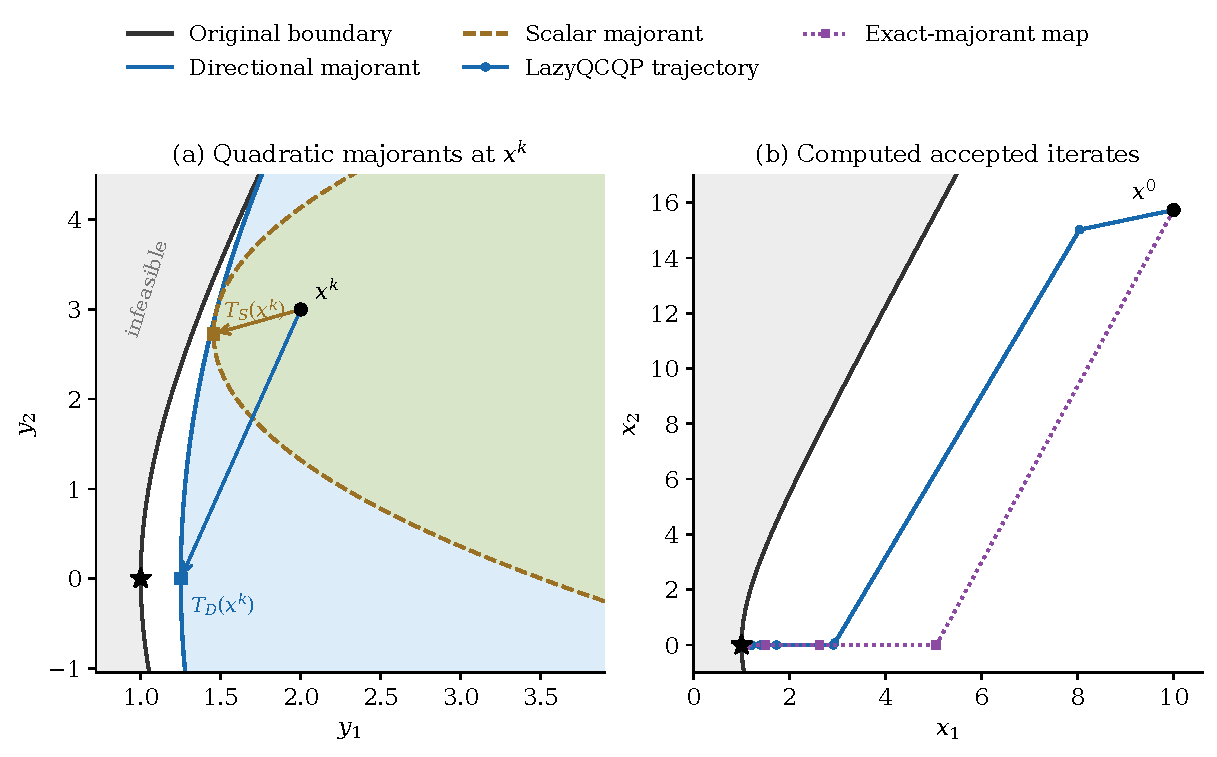
\includegraphics[width=\textwidth]{fig_favorable_geometry.pdf}
 \caption{First illustration, $\beta=0.1$. Left: directional and scalar
 exact inner models at $(2,3)$ and their minimizers. Right: the computed
 adaptive trajectory and separate exact-model reference. Grey denotes
 original infeasibility.}
 \label{fig:favorable-geometry}
\end{figure}

With $\beta=0.1$, all trajectories start at
$x^0=(10,15.732132722552274)^T$, where $g_\beta=-74.25$.
The adaptive construction starts scalar and retains a single normal
direction after its first accepted step. For intermediate comparisons,
the bound normal for $B=\{x:x_1\geq0\}$ is eliminated from stationarity:
\begin{equation}\label{eq:favorable-box-kkt}
 \begin{aligned}
 r_B&=\operatorname{dist}_\infty
       (-\nabla f-\lambda\nabla g_\beta,N_B(x)),\\
 \mathcal R_B&=\max\{[g_\beta]_+,r_B,
                     |\lambda g_\beta|,[-\lambda]_+\}.
 \end{aligned}
\end{equation}
Recorded quadratic multipliers are used without refitting. Final points
also pass the full original KKT test. Figure~\ref{fig:favorable-convergence}
shows the directional configuration reaching the common threshold first
for this start. The scalar trajectory has median tangent ratio
$0.909091$ over iterations 39--49, matching $10/11$.

\begin{figure}[!tb]
 \centering
 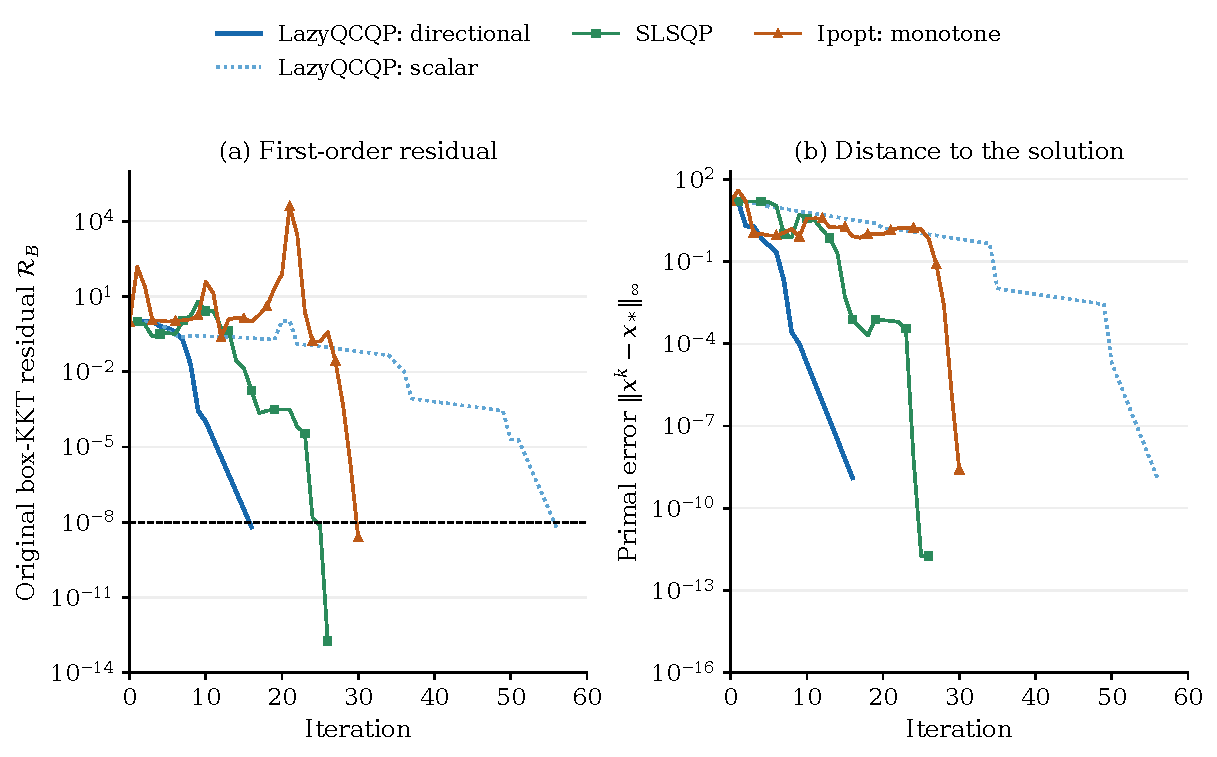
\includegraphics[width=\textwidth]{fig_favorable_convergence.pdf}
 \caption{Computed trajectories from the common start: original box-KKT
 residual and distance to the known solution. SLSQP points follow its
 accepted line-search iterates with their evolving subproblem multipliers.}
 \label{fig:favorable-convergence}
\end{figure}

A coordinate control, $u=x_1$, $w=\sqrt\beta x_2$, changes the scalar
model factor from $10/11$ to $1/2$ and its iteration count from 56 to
30; the directional configuration remains at 16 iterations. Every
final point passes the original-coordinate test. This separates
representation-dependent correction and stopping rules from equivalent
QCQP geometry; details appear in Supplement~\ref{supp:controlled-details}.

Extending $x_2$ to $v\in\mathbb R^{n-1}$ gives the radial family
\eqref{eq:radial-family}, with one negative Hessian direction and a
rank-one correction for every $n$. It retains the same two-dimensional
radial geometry. Figure~\ref{fig:radial-scaling} reports five
single-threaded, pinned solves per dimension, excluding startup and
problem preparation. Small cases where SLSQP is faster are included.
At $n=2000$, directional correction takes 16 iterations and 106.41 ms,
against 80 iterations and 426.54 ms for scalar correction; Ipopt and
SLSQP take 172.54 and 429.26 ms. The corresponding speedups are 1.62
and 4.03. These timings combine iteration counts, storage and sparse or
dense linear algebra; they measure this fixed radial structure.

\begin{figure}[!tb]
 \centering
 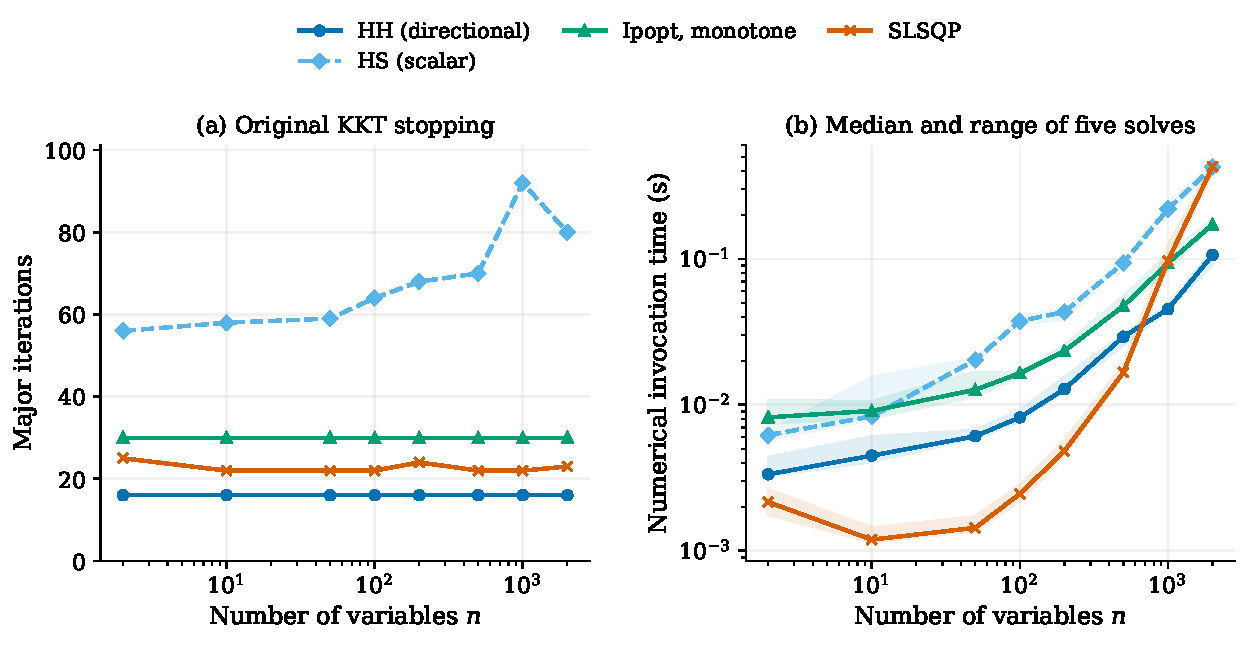
\includegraphics[width=\textwidth]{fig_radial_scaling_common_kkt.pdf}
 \caption{Radial family: major iterations and median numerical solve
 times. Bands span the five measured solves. HS is scalar and HH
 directional. All final points meet the original $10^{-8}$ KKT threshold.}
 \label{fig:radial-scaling}
\end{figure}

\subsection{An unavoidable tangent penalty}\label{sec:toy-geometry}
Changing one quadratic sign reverses the role of refinement. Consider
\begin{equation}\label{eq:paired-toys}
 \min_x\ \tfrac12\bigl((x_1-a)^2+x_2^2\bigr)
 \quad\text{subject to}\quad
 g_\pm(x)=1-x_1^2\pm x_2^2\leq0,\qquad a=0.1.
\end{equation}
Both problems have unique global solution $x^*=(1,0)^T$, value
$0.405$, multiplier $\lambda^*=0.45$, and the same feasible start
$(1.6,0.8)^T$. LICQ, strict complementarity and SOSC hold.

For circular exclusion $g_-$, the minimal spectral correction $2I$
gives the affine majorant
\begin{equation}\label{eq:circle-majorant}
 \widehat g_-(y;x)=1+\|x\|^2-2x^Ty,
 \qquad \widehat g_--g_-=\|y-x\|^2.
\end{equation}
Its exact-model map has
$DT_-(x^*)=\operatorname{diag}(0,0.9)$. On the tangent $e_2$,
\[
 H_T=0.1,\qquad E_T=0.9,\qquad\kappa=9,
 \qquad\rho(T_*)=0.9.
\]
The lower bound is attained: convexity requires $e_2^TM_-e_2\geq2$,
so $\kappa\geq\lambda^*2/H_T=9$, with equality for $M_-=2I$.
The exact reference converges from the stated feasible start;
Supplement~\ref{supp:controlled-details} gives the map and argument.
Here the majorant and first-order SQP constraint are the same
halfspace, while their objective curvatures differ: $I$ for the model
and the signed Lagrangian Hessian $aI$ for exact-Hessian SQP.

For hyperbolic exclusion $g_+$, negative curvature lies only in the
normal direction. The correction $\operatorname{diag}(2,0)$ gives
\begin{equation}\label{eq:hyperbola-majorant}
 \widehat g_+(y;x)=1+x_1^2-2x_1y_1+y_2^2,
 \qquad\widehat g_+-g_+=(y_1-x_1)^2.
\end{equation}
Its local exact map is
$T_+(x)=((x_1+x_1^{-1})/2,0)^T$, with $H_T=1.9$ and
$E_T=0$, hence quadratic normal error. Scalar correction instead gives
$E_T=0.9$, $B_T=2.8$ and factor $9/28$.
Figure~\ref{fig:toy-geometry} contrasts the models.

\begin{figure}[!tb]
 \centering
 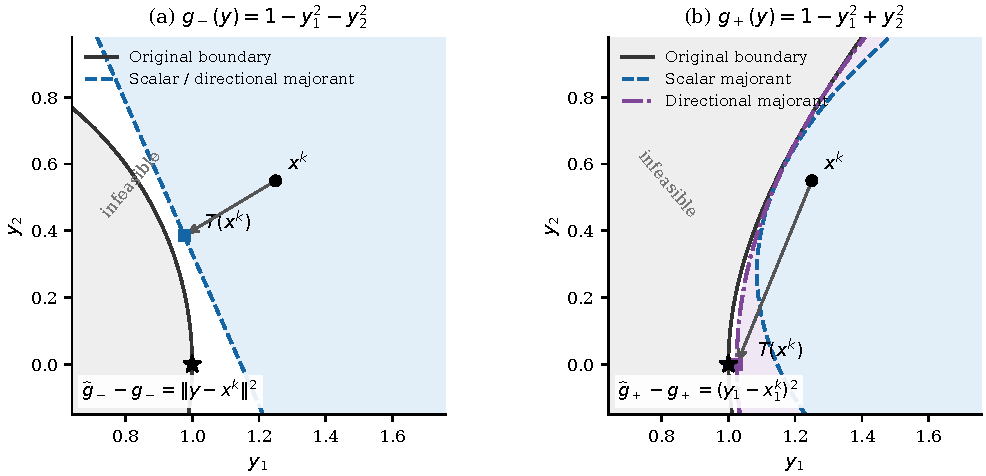
\includegraphics[width=\textwidth]{fig_toy_pair_geometry.pdf}
 \caption{Exact inner models at $(1.25,0.55)^T$. The directional
 hyperbolic correction releases the purple region. Arrows show exact
 model minimization; the star is the common solution.}
 \label{fig:toy-geometry}
\end{figure}

Figure~\ref{fig:toy-convergence} compares the computed Newton iterations
with exact-model references. On the circle, scalar and adaptive
trajectories coincide: 146 iterations with observed tangent factor
$0.9000$, against 147 for the exact model, seven for exact-Hessian SQP
and six for Ipopt. This behavior agrees with the forced tangent excess.
On the hyperbola it reduces the computed count from 20 to 14;
the exact directional reference takes five steps and Ipopt four.
The scalar tail ratio $0.321429$ matches $9/28$, while the exact
directional normal-error quotient approaches $1/2$.

\begin{figure}[!tb]
 \centering
 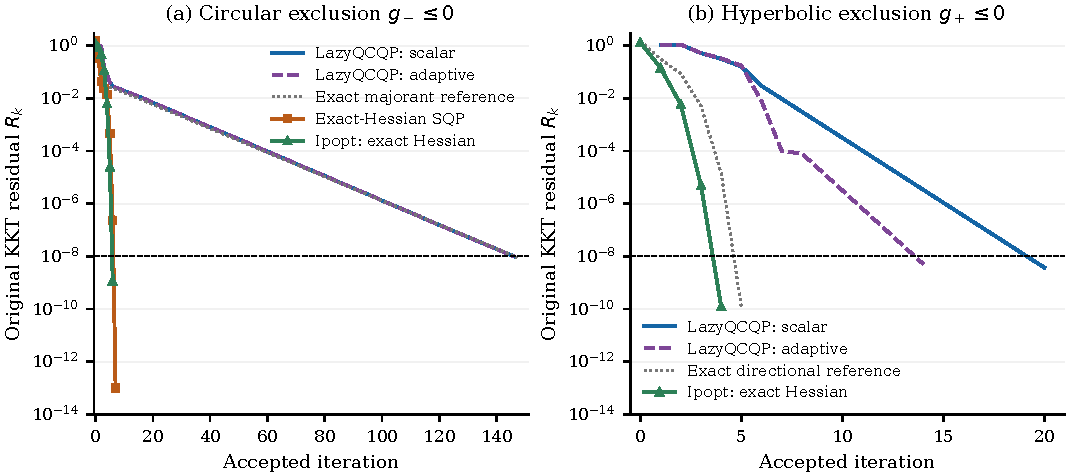
\includegraphics[width=\textwidth]{fig_toy_pair_convergence.pdf}
 \caption{Original KKT residuals from the common start. Solid and dashed
 curves are accepted LazyQCQP iterates; dotted curves minimize the
 analytical majorants exactly. The line marks $10^{-8}$.}
 \label{fig:toy-convergence}
\end{figure}

The adaptive hyperbolic trajectory reaches primal violation $0.493$
at its third accepted iterate: a single accepted Newton step need not
enforce the exact inner model. Its final normal-error ratio is $0.2$,
following the barrier schedule. This run and both Lazy configurations
in the first illustration finish after seven barrier reductions at
$\mu=1.28\times10^{-9}$, with stationarity about
$5.12\times10^{-9}$. The computed tail therefore illustrates the
barrier-forcing condition, alongside the curvature factors; the exact
map's quadratic rate applies when that perturbation becomes negligible.
\FloatBarrier
\section{Numerical assessment}\label{sec:protocol}
\subsection{Scope and common assessment}
The experiments examine how complete implementations of persistent
component models behave across different quadratic constraint structures.
They complement the geometric analysis: the controlled examples test its
local predictions, while the benchmark measures certificate counts,
computational cost and the stationary points found. Six native policies
are evaluated with each of MA27 and MUMPS on 4,078 continuous QCQPs from
28 collections. The corpus combines public instances, published generators
and application data \citep{GouldOrbanToint2015,PGLib2019,
BussieckDrudMeeraus2003,FuriniEtAl2019QPLIB,Friberg2016CBLIB}.
The 503 ASU radio-beamforming instances were constructed for this study
from DeepMIMO data \citep{Alkhateeb2019DeepMIMO}. Collection sources and
conversions are given in Supplementary Section~\ref{app:benchmark-sources}.

The regimes use the original quadratic constraints, before internal reductions. Regime I contains at least one quadratic
inequality and no quadratic equality; affine equalities and a quadratic
objective are allowed. Regime M contains both quadratic inequalities and
quadratic equalities. Regimes E and Q contain quadratic equalities and no
quadratic inequality, with an affine or constant objective in E and a
quadratic objective in Q. Bounds and affine constraints may occur in every
regime. Their sizes are 1,037, 797, 1,704 and 540, respectively. We focus on
I and M, where inequality convexification is present, and use E and Q to
examine the complementary equality-dominated settings.

Each configuration receives identical coefficients and the same raw primal
start. The limits are 7,200 seconds and 5,000 outer iterations; native
restoration has a shared allowance of 600 iterations across all phases.
Each task uses one numerical thread, with 22 concurrent tasks on an AMD
Ryzen Threadripper 7960X. Native linear algebra uses MA27 or MUMPS--METIS
\citep{AmestoyDuffExcellentKoster2001}. Both MUMPS implementations use
version 5.4.1; ordering, pivoting and memory controls are documented in
Supplementary Section~\ref{app:ipopt-protocol}. Exact internal reductions and native
recovery phases are charged to the same task. No external optimizer
supplies a new starting point.

A run succeeds when the independent evaluator verifies the primal, dual
and complementarity residuals in \eqref{eq:kkt-residual} on the complete
original QCQP, each at most $10^{-6}$, together with the input, start,
limits and the solver actually used. All planned instances remain in the
denominator. A run that does not supply such a certificate counts as a
failure to certify. This includes exhausted budgets and incomplete
execution records, as well as final points above tolerance; it does not
establish infeasibility. The supplementary results distinguish these
causes.

\subsection{Configurations and external reference}
R3 retains the exact objective and uses a scalar correction $\rho P_S$ on a component's Hessian
support $S$, or a spectral correction on small supports. The H/S quartet
combines support-scalar corrections and hybrid corrections of the form
$\rho P_S+\sum_\ell\beta_\ell u_\ell u_\ell^T$, $\beta_\ell\geq0$.
Table~\ref{tab:variant-definitions} summarizes the policies; further
mechanism details appear in Supplementary
Section~\ref{app:policy-mechanisms}.

\begin{table}[t]
\centering\small
\caption{Solver configurations. In H/S labels, the letters specify objective and
inequality corrections, in that order. Each row is evaluated with MA27 and
MUMPS.}
\label{tab:variant-definitions}
\begin{tabularx}{\linewidth}{@{}l>{\raggedright\arraybackslash}X>{\raggedright\arraybackslash}X@{}}
\toprule
Policy & Component corrections & Other defining mechanisms\\
\midrule
R3 & Exact objective; cached support-scalar or small-support spectral
inequality corrections. & Signed equality curvature; structural and
direction-accuracy safeguards; retains quadratically implied bound rows.\\
HH & Hybrid objective and inequalities. & Signed equality curvature;
common globalization, feasibility corrections and implied-bound removal.\\
HS & Hybrid objective; support-scalar inequalities. & As HH.\\
SH & Support-scalar objective; hybrid inequalities. & As HH.\\
SS & Support-scalar objective and inequalities. & Same controller as HH;
retains quadratically implied bound rows.\\
$SS_0$ & Ambient scalar corrections. & Equality linearization, proximal
curvature bound and scalar-control globalization.\\
\bottomrule
\end{tabularx}
\end{table}

The twelve policy--linear-solver combinations are separate experimental
configurations. During a run their mechanisms remain fixed.
R3 and HH also differ in globalization and safeguards, while $SS_0$ changes
equality treatment. Consequently, their coverage differences measure the
performance of complete policies. The H/S quartet shares its step
controller, but R3 and SS retain bound rows that HH, HS and SH remove
when implied by quadratic equalities. The reduction preserves the feasible set and
changes the barrier equations. On all 503 ASU MA27 cases, the latter
three policies remove 128 bound sides in 501 cases and 64 in two; SS
removes none. R3 likewise removes none in the 503 available ASU MA27
observations, with unchanged variable dimensions. The MUMPS implementation uses the same mode-dependent rule.
Thus comparisons involving SS combine curvature and preprocessing.
HH/HS and HH/SH share preprocessing, globalization and safeguards within
each linear-solver implementation. These comparisons therefore focus on
their component-correction choices.
MUMPS--METIS is the default linear solver of LazyQCQP and serves as its
native reference backend. The MA27 implementation uses the same native
policies and accuracy safeguards
with the settings in Supplementary
Section~\ref{app:ipopt-protocol}. We report its results as a linear-solver
sensitivity comparison.

The external reference is Ipopt 3.14.11 with exact Hessians and each of
MA27 and MUMPS \citep{WachterBiegler2006,IpoptOptions2026}. The principal
comparison uses its default monotone barrier strategy with stopping
settings aimed at the common original certificate: \texttt{tol}$=10^{-8}$,
\texttt{constr\_viol\_tol}, \texttt{dual\_inf\_tol} and
\texttt{compl\_inf\_tol}$=10^{-6}$, \texttt{acceptable\_iter}$=0$, and
\texttt{bound\_relax\_factor}$=0$. The time and iteration limits agree
with those above. These Ipopt options target comparable precision, but the independent
evaluator determines success because its residual definitions differ
from Ipopt's. The adaptive barrier strategy
with the same stopping settings supplies a sensitivity comparison for
both linear solvers on the complete corpus.

\begin{table}[t]
\centering\small
\caption{Original-KKT certificates by regime. All planned instances enter
the denominators. Ipopt uses certificate-matched stopping targets; its
monotone rows are the principal reference and its adaptive rows assess
barrier-strategy sensitivity. Column maxima are in bold.}
\label{tab:mega-regimes}
\setlength{\tabcolsep}{4pt}
\begin{tabular}{@{}llrrrrr@{}}
\toprule
Policy & Linear solver & I & M & E & Q & All\\
& & $N=1037$ & $N=797$ & $N=1704$ & $N=540$ & $N=4078$\\
\midrule
R3 & MA27 &996&\textbf{663}&1324&537&3520\\
HH & MA27 &888&661&1492&536&3577\\
HS & MA27 &889&622&1492&536&3539\\
SH & MA27 &887&661&1492&536&3576\\
SS & MA27 &889&660&1492&536&3577\\
$SS_0$ & MA27 &682&51&1248&519&2500\\
\addlinespace
R3 & MUMPS &\textbf{1026}&660&1314&\textbf{540}&3540\\
HH & MUMPS &895&660&\textbf{1527}&537&\textbf{3619}\\
HS & MUMPS &891&621&\textbf{1527}&537&3576\\
SH & MUMPS &894&660&\textbf{1527}&536&3617\\
SS & MUMPS &891&659&\textbf{1527}&536&3613\\
$SS_0$ & MUMPS &685&52&1249&519&2505\\
\midrule
Ipopt, monotone & MA27 &1008&438&1485&534&3465\\
Ipopt, monotone & MUMPS &1007&423&1153&536&3119\\
Ipopt, adaptive & MA27 &989&336&1373&537&3235\\
Ipopt, adaptive & MUMPS &989&310&1336&537&3172\\
\bottomrule
\end{tabular}
\end{table}

A separate stopping-rule diagnostic retains Ipopt's default termination
settings. Its positive exits fail the original certificate in 1,859 MA27
and 741 MUMPS cases, predominantly through complementarity. Those results
quantify agreement between termination and certification; they are not the
principal coverage comparison. Full option values, exit categories and
collection-level residuals appear in Supplementary
Section~\ref{app:ipopt-protocol}.

\subsection{Coverage and corpus composition}
In I, R3 has the highest native certificate count. With MUMPS it certifies
1,026/1,037 instances (98.9\%), against 1,007 (97.1\%) for monotone Ipopt.
The MA27 sensitivity comparison reverses this ordering: 996 certificates
for R3 against 1,008 for Ipopt. The adaptive Ipopt strategy certifies 989
cases with either linear solver. Table~\ref{tab:mega-regimes} gives all
policy counts.

In M, R3 certifies 660/797 cases with MUMPS against 423 for monotone Ipopt;
the MA27 counts are 663 and 438. ASU supplies 503 of these 797 problems.
R3, HH, SH and SS each certify 375 ASU cases with either linear solver,
compared with 337 for HS and none for the scalar control. Monotone Ipopt
certifies 214 with MUMPS and 212 with MA27. The difference extends beyond
ASU: on the remaining 294 mixed problems, R3 certifies 285 against 209
for monotone Ipopt with MUMPS, and 288 against 226 with MA27. Adaptive
Ipopt improves coverage on PGLib but reduces it on ASU, illustrating
collection-dependent effects of the barrier strategy. Failure causes are
reported in Supplementary Table~\ref{tab:failure-breakdown}.

In E, the H/S quartet has higher coverage than R3, but GasLib134 contributes
1,208 of the 1,704 cases. Removing this constant-objective feasibility
collection leaves 320/496 MUMPS certificates for both the quartet and
monotone Ipopt; with MA27, their counts are 284 and 300. Since objective
and inequality corrections vanish in E, these differences concern equality
handling, globalization and safeguards. In Q, every native configuration
certifies all 500 robot-arm problems. Only the remaining 40 cases
distinguish their coverage; R3 with MUMPS certifies all of them. Thus the
large aggregate counts in E and Q depend strongly on their dominant
collections.

These results compare complete policies on the specified corpus.
Supplementary Section~\ref{app:composition} reports rates after removing
the largest collection and under equal-family and equal-collection
weighting, which give each metadata family and each dataset equal weight,
respectively. These groups provide descriptive summaries of the corpus.

\subsection{Computational cost and stationary-point objectives}
Each configuration has one execution per instance under concurrent load.
Elapsed process time includes startup and resource monitoring, and excludes
independent auditing. Paired time ratios use common strict certificates;
we also restrict to pairs whose two times exceed one second, without
subtracting a startup constant. Figure~\ref{fig:performance-profiles}
compares all six native policies with monotone Ipopt, holding the linear
solver fixed in each panel. Following \citet{DolanMore2002}, times are
normalized by the fastest certified time; failure to certify receives an
infinite ratio. Every planned case remains in the denominator, including
those with no certificate.

\begin{figure}[t]
\centering
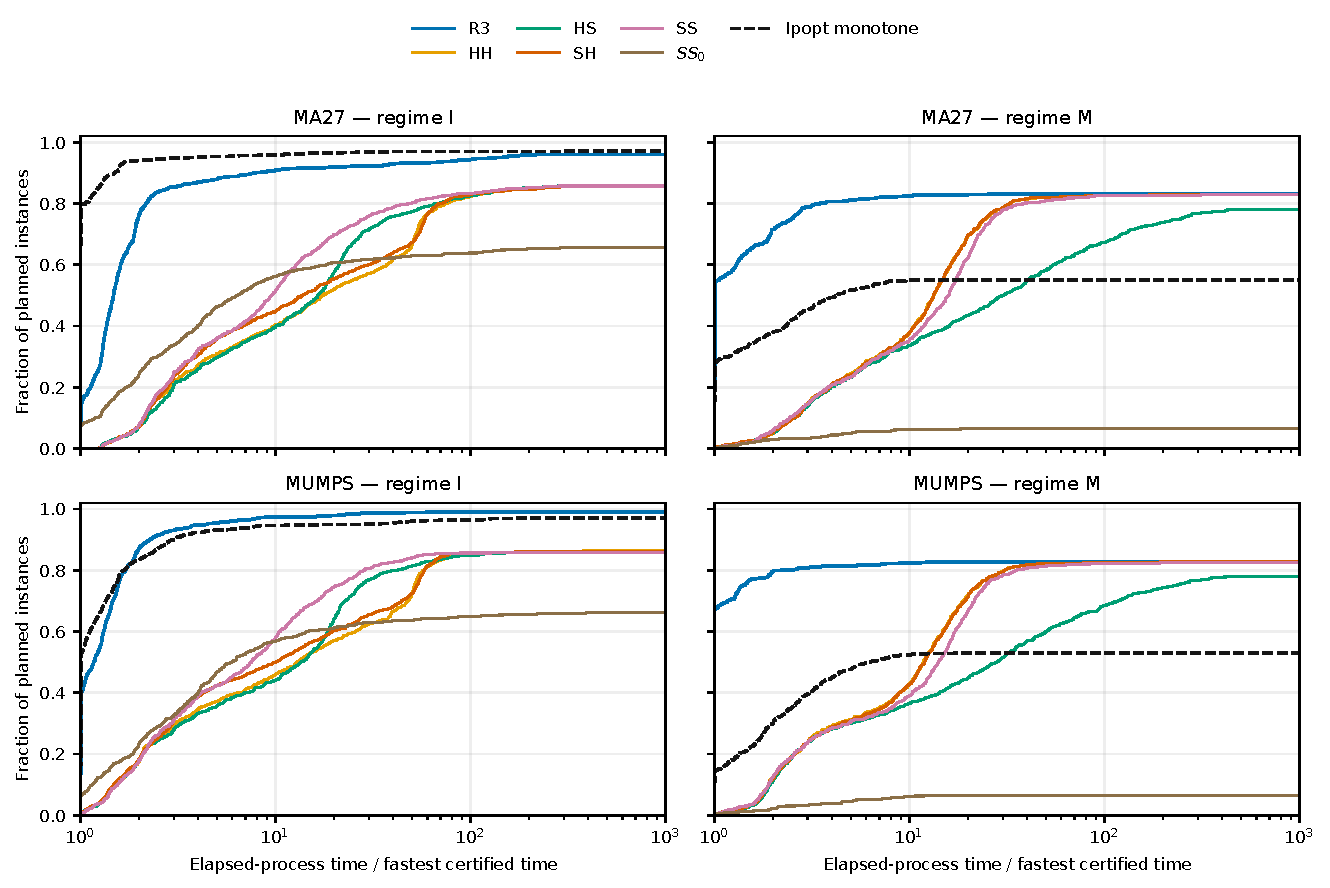
\includegraphics[width=\linewidth]{fig_aligned_core_performance_profiles.pdf}
\caption{Elapsed-process performance profiles in I and M. Rows hold
the linear solver fixed; columns hold the regime fixed. Each panel includes
all six native policies, monotone Ipopt with certificate-matched stopping
targets, and all planned cases. There is no objective-equivalence restriction.}
\label{fig:performance-profiles}
\end{figure}

For pairs whose two times exceed one second, the median R3/monotone-Ipopt
ratios with MUMPS are $0.34$ in I (81 pairs) and $0.48$ in M (75 pairs).
The MA27 sensitivity comparison gives $0.83$ (30 pairs) and $2.12$
(89 pairs). These conditional medians concern different cohorts;
Supplementary Sections~\ref{app:aligned-reference-results}
and~\ref{app:all-policy-comparisons} give their dispersion and all policy
comparisons.

A KKT certificate concerns stationarity. We therefore compare the
original minimization objectives on common strict certificates using
\[
\delta_f(A,B)=\frac{f_A-f_B}{\max\{1,|f_A|,|f_B|\}}.
\]
Negative values favor $A$. Lower/equivalent/higher counts use thresholds
$10^{-3}$ and $10^{-2}$; quartiles use the full common cohort. The original
objective and its constant are identical across configurations.

Table~\ref{tab:objective-core} separates ASU from the other mixed problems.
On ASU, R3's median gap to HH or SH is $18.64\%$, with a higher objective
in 372/375 common pairs at $10^{-3}$ under either linear solver. Its median
gap to monotone Ipopt is $15.93\%$ with MUMPS (214 pairs) and $15.17\%$
with MA27 (212 pairs). HH and SH have median gaps near zero to Ipopt. R3/SS has a near-zero signed median and a median absolute gap of
$0.79\%$. Outside ASU, the native and reference median gaps are near zero.
Full threshold counts and terminal residuals appear in Supplementary
Section~\ref{app:objective-accuracy}.

\begin{table}[t]
\centering\footnotesize
\setlength{\tabcolsep}{5pt}
\caption{Native stationary objectives in M: $\delta_f$(R3, comparison
policy), in percent, on common strict certificates. Entries give median
$[Q_1,Q_3]$ on the whole cohort. Each comparison holds the linear solver
fixed. ASU has 503 planned cases; the complement has 294.}
\label{tab:objective-core}
\begin{tabular}{@{}llrcr c@{}}
\toprule
Linear solver & Comparison & $N_{\rm ASU}$ & ASU gap (\%) & $N_{\rm rest}$ & Rest gap (\%)\\
\midrule
MA27 & HH &375&18.64 [11.87,25.47]&285&0.00 [0.00,0.00]\\
 & HS &337&17.79 [11.07,23.11]&284&0.00 [0.00,0.00]\\
 & SH &375&18.64 [11.87,25.47]&285&0.00 [0.00,0.00]\\
 & SS &375&0.00 [$-0.001$,2.04]&284&0.00 [0.00,0.00]\\
 & $SS_0$ &0&--&51&0.00 [0.00,0.00]\\
\addlinespace
MUMPS & HH &375&18.64 [11.87,25.47]&282&0.00 [0.00,0.00]\\
 & HS &337&17.79 [11.07,23.11]&281&0.00 [0.00,0.00]\\
 & SH &375&18.64 [11.87,25.47]&282&0.00 [0.00,0.00]\\
 & SS &375&0.00 [$-0.001$,2.04]&281&0.00 [0.00,0.00]\\
 & $SS_0$ &0&--&51&0.00 [0.00,0.00]\\
\bottomrule
\end{tabular}
\end{table}

The ASU objective differences involve different preprocessing: HH, HS and SH
remove quadratically implied bounds, while R3 and SS retain them.
Section~\ref{sec:bounds-persistence} isolates this rule. With common
preprocessing and a hybrid objective, HH certifies 375/503 ASU cases
against 337/503 for HS, adding 38 certificates without loss under either
linear solver. Their common-certificate objective median is nearly zero,
but 139/337 absolute gaps exceed $0.1\%$. Direct quartet comparisons and
their distinct paired cohorts are given in Supplementary
Section~\ref{app:quartet-direct-objectives}.

Representation sensitivity of central paths is established in linear
programming \citep{DezaNematollahiTerlaky2008,NematollahiTerlaky2008Touching};
decomposition choices also affect global QCQP algorithms
\citep{VanVoorhisAlKhayyal2003,ZhengSunLi2011}. Here the comparisons concern
attained stationary objectives.

Supplementary Section~\ref{app:published-reference-values} compares matched
QPLIB and MINLPLib facility-location objectives with published reference
points. With either linear solver,
R3's median relative objective gap to the QPLIB reference points is $0.02077\%$ on 47/49 certificates, against
$0.0001454\%$ on 48/49 for monotone Ipopt; the supplement gives the full
distributions and facility results. The ASU comparisons use objectives
attained by the paired solvers.

\subsection{Controlled refinement and curvature diagnostics}
A separate $2\times2$ experiment crosses fixed or adaptive inequality
corrections with two globalization policies under each linear solver,
holding the objective, initial corrections, bound preprocessing and
safeguards fixed. Its 14,672 observations include 12,970 original
certificates and 189 incomplete records. The specified primary comparison
gives net certificate gains of zero with MA27 and one with MUMPS among
complete records; the bounds including incomplete records span both signs.
On common certificates with both times above one second, median
adaptive/fixed time ratios are 1.01--1.06. The ASU comparisons report
lower iteration counts and median process-time ratios above one. Supplementary
Section~\ref{app:controlled-refinement} reports the full comparisons;
Section~\ref{app:curvature-diagnostics} discusses the limits of benchmark
curvature diagnostics as estimates of asymptotic factors.

\subsection{Controlled bound removal and correction reuse}\label{sec:bounds-persistence}
The ASU ablation crosses R3, SS and HH with retention or removal of
quadratically implied bounds under both linear solvers: $503\times3\times2
\times2=6{,}036$ observations. A common executable, identical inputs and
raw starts, and unchanged policies and limits isolate the bound-removal
rule; certification includes all original bounds. Table~\ref{tab:asu-bounds-controlled}
reports this separate experiment, with objective gaps on the cohort
certified by all six configurations within each backend. Removal lowers
objectives in 299--303 cases per row at threshold $10^{-3}$, with median
gaps of 15.7--16.2\%. After removal, R3 obtains 63 fewer certificates under each backend;
these cases reach the 5,000-iteration limit. SS obtains 40 or 41 fewer,
and HH retains its 374 certificates. Every certificate obtained after
removal is also obtained with the bounds retained. The campaign records
4,285 strict, 1,729 nonstrict and 22 indeterminate results. Bound removal
changes both attained objectives and certificate counts in this experiment. Supplementary Section~\ref{supp:asu-bounds}
gives the controls and incomplete-record diagnostics.

\begin{table}[t]
\centering\small
\caption{Controlled ASU bound removal. Coverage is strict certificates out
of 503. Objective medians use the same six-configuration common cohort
within each backend; gaps are $100\delta_f(\mathrm{keep},\mathrm{remove})$.}
\label{tab:asu-bounds-controlled}
\begin{tabular}{@{}llrrrc@{}}
\toprule
Linear solver & Policy & Keep & Remove & Common $N$ & Median gap (\%)\\
\midrule
MA27 & R3 & 375 & 312 & 305 & 16.24\\
     & SS & 374 & 334 & 305 & 15.69\\
     & HH & 374 & 374 & 305 & 16.21\\
\addlinespace
MUMPS & R3 & 375 & 312 & 304 & 16.18\\
      & SS & 374 & 333 & 304 & 15.68\\
      & HH & 374 & 374 & 304 & 16.19\\
\bottomrule
\end{tabular}
\end{table}

A second ablation compares reuse with rebuilding the same deterministic
DC correction on 12 selected I/M instances under both linear solvers.
The 72 preliminary runs verify matching trajectories and record 4,638
constructions with rebuild and 25 with reuse. Three repetitions per mode
give 144 timed runs, all original-KKT certified, with matching outputs
and work counters.
Sequential, single-thread process times monitored for other CPU activity
give median reuse/rebuild ratios of 0.849 with MA27 and 0.853 with MUMPS;
reuse is faster on all 24 pairs. This measures avoided
construction cost at unchanged numerical behavior on the selected cases.
Supplementary Section~\ref{supp:persistence} gives the selection, controls
and timing protocol.
\FloatBarrier
\section{Discussion and conclusion}
The tangent-excess bound quantifies the local convergence cost forced
by valid componentwise convexification. The examples show that this bound
can be attained. The normal-space criterion
characterizes when corrections can avoid that cost. Established
sensitivity formulas give the spectral factor $\kappa/(1+\kappa)$, which
the controlled QCQPs reproduce.

LazyQCQP combines reusable DC corrections, signed equality curvature and
original-function step tests. The specified LazyQCQP-F algorithm has a
global stationarity guarantee under boundedness, uniform regularity,
reduced coercivity, successful restoration and barrier continuation.
Near a regular KKT limit, a small enough
curvature threshold removes additional diagonal regularization; the local
rate also requires limiting corrections, full steps and vanishing forcing
errors.

R3 has the highest native certificate counts in the inequality regime;
its relative coverage against monotone Ipopt varies with the linear solver.
Higher mixed-regime coverage is accompanied by positive median objective
gaps on ASU relative to monotone Ipopt.
Controlled bound removal lowers attained objectives and reduces certificate
counts for R3 and SS. Correction reuse reduces construction work at
unchanged numerical behavior. Adaptive refinement changes trajectories,
with comparable certificate counts in the controlled experiment. These
comparisons reflect the corpus composition and the complete algorithmic policies.

These are local stationarity results. Certified feasible points can supply
incumbents to global optimization methods.

\section*{Statements and Declarations}
\paragraph{Funding.}
The author received no specific funding for this work.

\paragraph{Competing interests.}
The author declares no competing interests.

\paragraph{Code and data availability.}
The project repository for the solver, benchmark inputs, generators and
analysis scripts is \url{https://github.com/francoisakoa/lazyqcqp}.
The supplement records the sources and model conversions used in the
computational study.

\paragraph{AI-assisted work.}
Under the author’s direction, ChatGPT (OpenAI) and Claude (Anthropic)
assisted in language refinement, checking of derivations, and code
development. The author verified all results and is responsible for the
final content.

\FloatBarrier
\begingroup\small\setlength{\bibsep}{2pt}\begin{thebibliography}{99}

\providecommand{\natexlab}[1]{#1}
\providecommand{\url}[1]{\texttt{#1}}
\expandafter\ifx\csname urlstyle\endcsname\relax
  \providecommand{\doi}[1]{doi: #1}\else
  \providecommand{\doi}{doi: \begingroup \urlstyle{rm}\Url}\fi


\bibitem[Akoa(2005)]{Akoa2005Thesis}
Fran\c{c}ois~Bertrand Akoa.
\newblock \emph{Approches de points int{\'e}rieurs et de la programmation {DC}
  en optimisation non convexe. Codes et simulations num{\'e}riques
  industrielles}.
\newblock Doctoral thesis in applied mathematics, Institut national des
  sciences appliqu{\'e}es de Rouen, Rouen, France, January 2005.
\newblock URL \url{https://theses.hal.science/tel-00008475}.
\newblock Defended on 27 January 2005. HAL: tel-00008475.

\bibitem[Alkhateeb(2019)]{Alkhateeb2019DeepMIMO}
Ahmed Alkhateeb.
\newblock DeepMIMO: a generic deep learning dataset for millimeter wave and massive MIMO applications.
\newblock arXiv:1902.06435, 2019.
\newblock \url{https://arxiv.org/abs/1902.06435}.

\bibitem[Amestoy et~al.(2001)Amestoy, Duff, {L'Excellent}, and
  Koster]{AmestoyDuffExcellentKoster2001}
Patrick~R. Amestoy, Iain~S. Duff, Jean-Yves {L'Excellent}, and Jacko Koster.
\newblock A fully asynchronous multifrontal solver using distributed dynamic
  scheduling.
\newblock \emph{SIAM Journal on Matrix Analysis and Applications}, 23\penalty0
  (1):\penalty0 15--41, 2001.
\newblock \url{https://doi.org/10.1137/S0895479899358194}.

\bibitem[Auslender et~al.(2010)Auslender, Shefi, and
  Teboulle]{AuslenderShefiTeboulle2010}
Alfred Auslender, Ron Shefi, and Marc Teboulle.
\newblock A moving balls approximation method for a class of smooth constrained
  minimization problems.
\newblock \emph{SIAM Journal on Optimization}, 20\penalty0 (6):\penalty0
  3232--3259, 2010.
\newblock \url{https://doi.org/10.1137/090763317}.

\bibitem[Babaeinejadsarookolaee et~al.(2019)Babaeinejadsarookolaee, Birchfield,
  Christie, Coffrin, DeMarco, Diao, Ferris, Fliscounakis, Greene, Huang, Josz,
  Korab, Lesieutre, Maeght, Mak, Molzahn, Overbye, Panciatici, Park, Snodgrass,
  Tbaileh, {Van Hentenryck}, and Zimmerman]{PGLib2019}
Sogol Babaeinejadsarookolaee, Adam Birchfield, Richard~D. Christie, Carleton
  Coffrin, Christopher DeMarco, Ruisheng Diao, Michael Ferris, Stephane
  Fliscounakis, Scott Greene, Renke Huang, Cedric Josz, Roman Korab, Bernard
  Lesieutre, Jean Maeght, Terrence W.~K. Mak, Daniel~K. Molzahn, Thomas~J.
  Overbye, Patrick Panciatici, Byungkwon Park, Jonathan Snodgrass, Ahmad
  Tbaileh, Pascal {Van Hentenryck}, and Ray Zimmerman.
\newblock The power grid library for benchmarking {AC} optimal power flow
  algorithms, 2019.
\newblock URL \url{https://arxiv.org/abs/1908.02788}.
\newblock Revised 4 January 2021.

\bibitem[Bussieck et~al.(2003)Bussieck, Drud, and
  Meeraus]{BussieckDrudMeeraus2003}
Michael~R. Bussieck, Arne~Stolbjerg Drud, and Alexander Meeraus.
\newblock {MINLPLib}---a collection of test models for mixed-integer nonlinear
  programming.
\newblock \emph{INFORMS Journal on Computing}, 15\penalty0 (1):\penalty0
  114--119, 2003.
\newblock \url{https://doi.org/10.1287/ijoc.15.1.114.15159}.

\bibitem[COIN-OR Ipopt project(2026)]{IpoptOptions2026}
COIN-OR Ipopt project.
\newblock Ipopt options.
\newblock Software documentation, consulted 8 November 2026.
\newblock \url{https://coin-or.github.io/Ipopt/OPTIONS.html}.

\bibitem[Dennis and Mor{\'e}(1974)]{DennisMore1974}
John~E. Dennis, Jr. and Jorge~J. Mor{\'e}.
\newblock A characterization of superlinear convergence and its application to
  quasi-{Newton} methods.
\newblock \emph{Mathematics of Computation}, 28\penalty0 (126):\penalty0
  549--560, 1974.
\newblock \url{https://doi.org/10.1090/S0025-5718-1974-0343581-1}.

\bibitem[Dolan and Mor{\'e}(2002)]{DolanMore2002}
Elizabeth~D. Dolan and Jorge~J. Mor{\'e}.
\newblock Benchmarking optimization software with performance profiles.
\newblock \emph{Mathematical Programming}, 91\penalty0 (2):\penalty0 201--213,
  2002.
\newblock \url{https://doi.org/10.1007/s101070100263}.

\bibitem[Friberg(2016)]{Friberg2016CBLIB}
Henrik A. Friberg.
\newblock CBLIB 2014: a benchmark library for conic mixed-integer and continuous optimization.
\newblock \emph{Mathematical Programming Computation}, 8(2):191--214, 2016.
\newblock \url{https://doi.org/10.1007/s12532-015-0092-4}.

\bibitem[Fukushima et~al.(2003)Fukushima, Luo, and
  Tseng]{FukushimaLuoTseng2003}
Masao Fukushima, Zhi-Quan Luo, and Paul Tseng.
\newblock A sequential quadratically constrained quadratic programming method
  for differentiable convex minimization.
\newblock \emph{SIAM Journal on Optimization}, 13\penalty0 (4):\penalty0
  1098--1119, 2003.
\newblock \url{https://doi.org/10.1137/S1052623401398120}.

\bibitem[Furini et~al.(2019)]{FuriniEtAl2019QPLIB}
Fabio Furini, Emiliano Traversi, Pietro Belotti, Antonio Frangioni, Ambros Gleixner,
Nick Gould, Leo Liberti, Andrea Lodi, Ruth Misener, Hans Mittelmann,
Nikolaos V. Sahinidis, Stefan Vigerske, and Angelika Wiegele.
\newblock QPLIB: a library of quadratic programming instances.
\newblock \emph{Mathematical Programming Computation}, 11:237--265, 2019.
\newblock \url{https://doi.org/10.1007/s12532-018-0147-4}.

\bibitem[Gould et~al.(2015)Gould, Orban, and Toint]{GouldOrbanToint2015}
Nicholas I.~M. Gould, Dominique Orban, and Philippe~L. Toint.
\newblock {CUTEst}: a constrained and unconstrained testing environment with
  safe threads for mathematical optimization.
\newblock \emph{Computational Optimization and Applications}, 60\penalty0
  (3):\penalty0 545--557, 2015.
\newblock \url{https://doi.org/10.1007/s10589-014-9687-3}.

\bibitem[Higham(1988)]{Higham1988}
Nicholas~J. Higham.
\newblock Computing a nearest symmetric positive semidefinite matrix.
\newblock \emph{Linear Algebra and its Applications}, 103:\penalty0 103--118,
  1988.
\newblock \url{https://doi.org/10.1016/0024-3795(88)90223-6}.

\bibitem[Horn and Johnson(2013)]{HornJohnson2013}
Roger~A. Horn and Charles~R. Johnson.
\newblock \emph{Matrix Analysis}.
\newblock Cambridge University Press, Cambridge, 2 edition, 2013.
\newblock ISBN 9780521839402.
\newblock \url{https://doi.org/10.1017/CBO9781139020411}.

\bibitem[Hunter and Lange(2004)]{HunterLange2004}
David~R. Hunter and Kenneth Lange.
\newblock A tutorial on MM algorithms.
\newblock \emph{The American Statistician}, 58(1):30--37, 2004.
\newblock \url{https://doi.org/10.1198/0003130042836}.

\bibitem[{Le Thi} and {Pham Dinh}(2018)]{LeThiPhamDinh2018}
Hoai~An {Le Thi} and Tao {Pham Dinh}.
\newblock {DC} programming and {DCA}: thirty years of developments.
\newblock \emph{Mathematical Programming}, 169\penalty0 (1):\penalty0 5--68,
  2018.
\newblock \url{https://doi.org/10.1007/s10107-018-1235-y}.

\bibitem[Lipp and Boyd(2016)]{LippBoyd2016}
Thomas Lipp and Stephen Boyd.
\newblock Variations and extension of the convex--concave procedure.
\newblock \emph{Optimization and Engineering}, 17\penalty0 (2):\penalty0
  263--287, 2016.
\newblock \url{https://doi.org/10.1007/s11081-015-9294-x}.

\bibitem[Marks and Wright(1978)]{MarksWright1978}
Barry~R. Marks and Gordon~P. Wright.
\newblock Technical note---a general inner approximation algorithm for
  nonconvex mathematical programs.
\newblock \emph{Operations Research}, 26\penalty0 (4):\penalty0 681--683, 1978.
\newblock \url{https://doi.org/10.1287/opre.26.4.681}.

\bibitem[Messerer et~al.(2021)Messerer, Baumg\"artner, and Diehl]{MessererBaumgaertnerDiehl2021}
Florian Messerer, Katrin Baumg\"artner, and Moritz Diehl.
\newblock Survey of sequential convex programming and generalized
  Gauss--Newton methods.
\newblock \emph{ESAIM: Proceedings and Surveys}, 71:64--88, 2021.
\newblock \url{https://doi.org/10.1051/proc/202171107}.

\bibitem[{Pham Dinh} and {Le Thi}(1998)]{PhamDinhLeThi1998}
Tao {Pham Dinh} and Hoai~An {Le Thi}.
\newblock A {D.C.} optimization algorithm for solving the trust-region
  subproblem.
\newblock \emph{SIAM Journal on Optimization}, 8\penalty0 (2):\penalty0
  476--505, 1998.
\newblock \url{https://doi.org/10.1137/S1052623494274313}.

\bibitem[{Pham Dinh} et~al.(2008){Pham Dinh}, {Le Thi}, and
  Akoa]{PhamDinhLeThiAkoa2008}
Tao {Pham Dinh}, Hoai~An {Le Thi}, and Fran{\c c}ois Akoa.
\newblock Combining {DCA} ({DC} algorithms) and interior point techniques for
  large-scale nonconvex quadratic programming.
\newblock \emph{Optimization Methods and Software}, 23\penalty0 (4):\penalty0
  609--629, 2008.
\newblock \url{https://doi.org/10.1080/10556780802263990}.

\bibitem[Solodov(2004)]{Solodov2004}
Mikhail~V. Solodov.
\newblock On the sequential quadratically constrained quadratic programming
  methods.
\newblock \emph{Mathematics of Operations Research}, 29\penalty0 (1):\penalty0
  64--79, 2004.
\newblock \url{https://doi.org/10.1287/moor.1030.0069}.

\bibitem[W\"achter and Biegler(2005)]{WachterBiegler2005Global}
Andreas W\"achter and Lorenz~T. Biegler.
\newblock Line search filter methods for nonlinear programming:
  motivation and global convergence.
\newblock \emph{SIAM Journal on Optimization}, 16(1):1--31, 2005.
\newblock \url{https://doi.org/10.1137/S1052623403426556}.

\bibitem[W{\"a}chter and Biegler(2006)]{WachterBiegler2006}
Andreas W{\"a}chter and Lorenz~T. Biegler.
\newblock On the implementation of an interior-point filter line-search
  algorithm for large-scale nonlinear programming.
\newblock \emph{Mathematical Programming}, 106\penalty0 (1):\penalty0 25--57,
  2006.
\newblock \url{https://doi.org/10.1007/s10107-004-0559-y}.

\bibitem[Sherali and Tuncbilek(1992)]{SheraliTuncbilek1992}
Hanif D. Sherali and Cihan H. Tuncbilek.
\newblock A global optimization algorithm for polynomial programming problems using a Reformulation-Linearization Technique.
\newblock \emph{Journal of Global Optimization}, 2:101--112, 1992.
\newblock \url{https://doi.org/10.1007/BF00121304}.

\bibitem[Lasserre(2001)]{Lasserre2001}
Jean B. Lasserre.
\newblock Global optimization with polynomials and the problem of moments.
\newblock \emph{SIAM Journal on Optimization}, 11(3):796--817, 2001.
\newblock \url{https://doi.org/10.1137/S1052623400366802}.

\bibitem[Tawarmalani and Sahinidis(2005)]{TawarmalaniSahinidis2005}
Mohit Tawarmalani and Nikolaos V. Sahinidis.
\newblock A polyhedral branch-and-cut approach to global optimization.
\newblock \emph{Mathematical Programming}, 103:225--249, 2005.
\newblock \url{https://doi.org/10.1007/s10107-005-0581-8}.

% Published references verified against primary publisher records, 2026-11-09.
% Draft additions only: choose the references cited by the final text.
% Park--Boyd (working draft) and Akoa (unpublished manuscript) are given in
% attribution_snippets_R12.tex, following the journal's unpublished-work rule.

\bibitem[{Le Thi}(2000)]{LeThi2000Ellipsoids}
Hoai~An {Le Thi}.
\newblock An efficient algorithm for globally minimizing a quadratic function
  under convex quadratic constraints.
\newblock \emph{Mathematical Programming}, 87(3):401--426, 2000.
\newblock \url{https://doi.org/10.1007/s101070050003}.

\bibitem[{Le Thi} et~al.(2014){Le Thi}, Huynh, and {Pham Dinh}]{LeThiHuynhPhamDinh2014}
Hoai~An {Le Thi}, Van~Ngai Huynh, and Tao {Pham Dinh}.
\newblock DC programming and DCA for general DC programs.
\newblock In \emph{Advanced Computational Methods for Knowledge Engineering},
  volume 282 of \emph{Advances in Intelligent Systems and Computing},
  pages 15--35. Springer, 2014.
\newblock \url{https://doi.org/10.1007/978-3-319-06569-4_2}.

\bibitem[{Le Thi} et~al.(2012){Le Thi}, {Pham Dinh}, and Huynh]{LeThiPhamDinhHuynh2012}
Hoai~An {Le Thi}, Tao {Pham Dinh}, and Huynh~Van Ngai.
\newblock Exact penalty and error bounds in DC programming.
\newblock \emph{Journal of Global Optimization}, 52(3):509--535, 2012.
\newblock \url{https://doi.org/10.1007/s10898-011-9765-3}.
% Full third-author display name retained exactly as on the publisher page.

\bibitem[{Le Thi} et~al.(2011){Le Thi}, {Pham Dinh}, and Nguyen]{LeThiPhamDinhYen2011}
Hoai~An {Le Thi}, Tao {Pham Dinh}, and Nguyen~Dong Yen.
\newblock Properties of two DC algorithms in quadratic programming.
\newblock \emph{Journal of Global Optimization}, 49(3):481--495, 2011.
\newblock \url{https://doi.org/10.1007/s10898-010-9573-1}.
% Full third-author display name retained exactly as on the publisher page.

\bibitem[Lu et~al.(2022)Lu, Sun, and Zhou]{LuSunZhou2022}
Zhaosong Lu, Zhe Sun, and Zirui Zhou.
\newblock Penalty and augmented Lagrangian methods for constrained DC programming.
\newblock \emph{Mathematics of Operations Research}, 47(3):2260--2285, 2022.
\newblock \url{https://doi.org/10.1287/moor.2021.1207}.

\bibitem[{Pham Dinh} and {Le Thi}(1996)]{PhamDinhLeThi1996}
Tao {Pham Dinh} and Hoai~An {Le Thi}.
\newblock Difference of convex functions optimization algorithms (DCA) for
  globally minimizing nonconvex quadratic forms on Euclidean balls and spheres.
\newblock \emph{Operations Research Letters}, 19(5):207--216, 1996.
\newblock \url{https://doi.org/10.1016/S0167-6377(96)00036-3}.

\bibitem[Van~Voorhis and Al-Khayyal(2003)]{VanVoorhisAlKhayyal2003}
Tim {Van Voorhis} and Faiz~A. Al-Khayyal.
\newblock Difference of convex solution of quadratically constrained
  optimization problems.
\newblock \emph{European Journal of Operational Research}, 148(2):349--362, 2003.
\newblock \url{https://doi.org/10.1016/S0377-2217(02)00432-0}.

\bibitem[Zheng et~al.(2011)Zheng, Sun, and Li]{ZhengSunLi2011}
X.~J. Zheng, X.~L. Sun, and D.~Li.
\newblock Nonconvex quadratically constrained quadratic programming: best D.C.
  decompositions and their SDP representations.
\newblock \emph{Journal of Global Optimization}, 50(4):695--712, 2011.
\newblock \url{https://doi.org/10.1007/s10898-010-9630-9}.

% Verified against publisher metadata and primary full texts, 2026-11-09 UTC.
\bibitem[Deza et~al.(2008)Deza, Nematollahi, and Terlaky]{DezaNematollahiTerlaky2008}
Antoine Deza, Eissa Nematollahi, and Tam\'as Terlaky.
\newblock How good are interior point methods? Klee--Minty cubes tighten
  iteration-complexity bounds.
\newblock \emph{Mathematical Programming}, 113(1):1--14, 2008.
\newblock \url{https://doi.org/10.1007/s10107-006-0044-x}.

\bibitem[Nematollahi and Terlaky(2008)]{NematollahiTerlaky2008Touching}
Eissa Nematollahi and Tam\'as Terlaky.
\newblock A redundant Klee--Minty construction with all the redundant
  constraints touching the feasible region.
\newblock \emph{Operations Research Letters}, 36(4):414--418, 2008.
\newblock \url{https://doi.org/10.1016/j.orl.2008.02.004}.

\end{thebibliography}\endgroup
\end{document}
